% this file is called up by thesis.tex
% content in this file will be fed into the main document

\chapter{Replacement for Graph Community Detection Step} % top level followed by section, subsection
\label{cha:gcn}
% ----------------------- contents from here ------------------------
% 

This chapter presents the replacement created using a Graph
Convolusional Neural Network (GCN) as proposed by Kipf et al. for the
\emph{Graph Community Detection Step} of the Karas pipeline (see
\ref{cha:karas-pipeline}). It is observed that a GCN is able to
classify noise and event nodes very well, even in extremely skewed
datasets with less than 10 event nodes. The chapter begins with an
overview of GCNs and how they have been applied to this problem. The
data preparation, visualization and model evaluation are touched upon
next. The chapter concludes with discussion of the results.

\section{Primer on Graph Convolusional Neural Networks}
\label{sec:gcn-primer}

GCNs are designed to operate on data consisting of entities and their
relations, commonly referred to as \emph{graphs}. A graph $G = (V, E)$
consists of a set \emph{nodes (V)} and a set of \emph{edges (E)}. Each
node may or may not be connected to one or many nodes, these are
referred to as the \emph{neighbors} of the node. A graph with all
nodes connected to one another is called a \emph{fully connected
graph}. An edge may have attributes associated with it, the two most
common attributes being \emph{weight} and \emph{direction}. An edge
$(u, v) \in E$ between two nodes \emph{u} and \emph{v} may be
\emph{directed} which denotes a sense of hierarchy amongst the nodes,
an example being a graph which models how Twitter users follow one
another. An edge may also \emph{undirected} such as a graph which
models the friendship amongst the users of a social network (since
friendship is mutual). An edge may also have a weight to signify a
stronger or weaker connection amongst nodes. Nodes may also posses
attributes associated with themselves, commonly known as \emph{node
embeddings}. The complexity of the node embedding may range from a
simple scalar quantity to a multi-dimensional tensor, and depends on
the dataset and how the practitioner wishes to sculpt the graph.

Graphs are primarily classified into two variants namely
\emph{homogeneous} and \emph{heterogeneous} graphs. Homogeneous graphs
have the same type of entities and relations represented as nodes and
edges respectively. For example, a graph representing the social
network consisting of people and their connections is a homogeneous
graph. In contrast, Heterogeneous graph consist of different types of
nodes and edges. For example, a graph representing a person's likes
and dislikes in regards to food items. Here, two entities, namely
people and food are represented as nodes. The edges also come in two
variants ie. a 'like' and a 'dislike'.

% TODO illustrate the paradigm
GCNs learn by utilizing a message passing paradigm which is summarized
in Figure \ref{gcn-message-passing}. During each training epoch, all
nodes propagate their embedding to their neighbors. The collected
embeddings are then aggregated (for example using a sum, difference or
mean) which becomes the new embedding for the node. This procedure is
done for all nodes of the graph, for each training epoch. The number
of layers in the network determine how far the messages are sent. For
example, for a network with a single layer, each node aggregates the
embeddings from their immediate neighbors. With 2 layers, the node
also aggregates embeddings from the neighbors of it's immediate
neighbors and so forth.

%% \subsection{GNN and it's Variants}

%% GNNs have two primary applications.

%% \begin{enumerate}
%% \item \textbf{Node classification}. This is a semi-supervised learning
%%   setting (although it can also be used in a supervised setting).
%%   Given a graph with nodes associated with a label, the network can be
%%   used to predict the label of unseen nodes.
%% \item \textbf{Graph classification}. In this approach, the network is
%%   trained using several graphs each associated with a label. The
%%   network can then be used to predict the label of an unseen graph.
%% \end{enumerate}


\section{Data Preparation}
\label{sec:gcn-data-prep}

The graphs for the testing and training of the network are constructed
from a combination of the main dataset and a modified version of the
MLP dataset, Figure \ref{fig:gcn-data} illustrates this procedure. A
fully connected graph is constructed, and its node embeddings and node
labels are derived from the main dataset. Each node is thus assigned a
$(x,y,z,t)$ vector as it's node embedding. The node is assigned a
label of 1 if it is an event hit, else a label of 0.

\begin{figure}[htb]
  \centering
  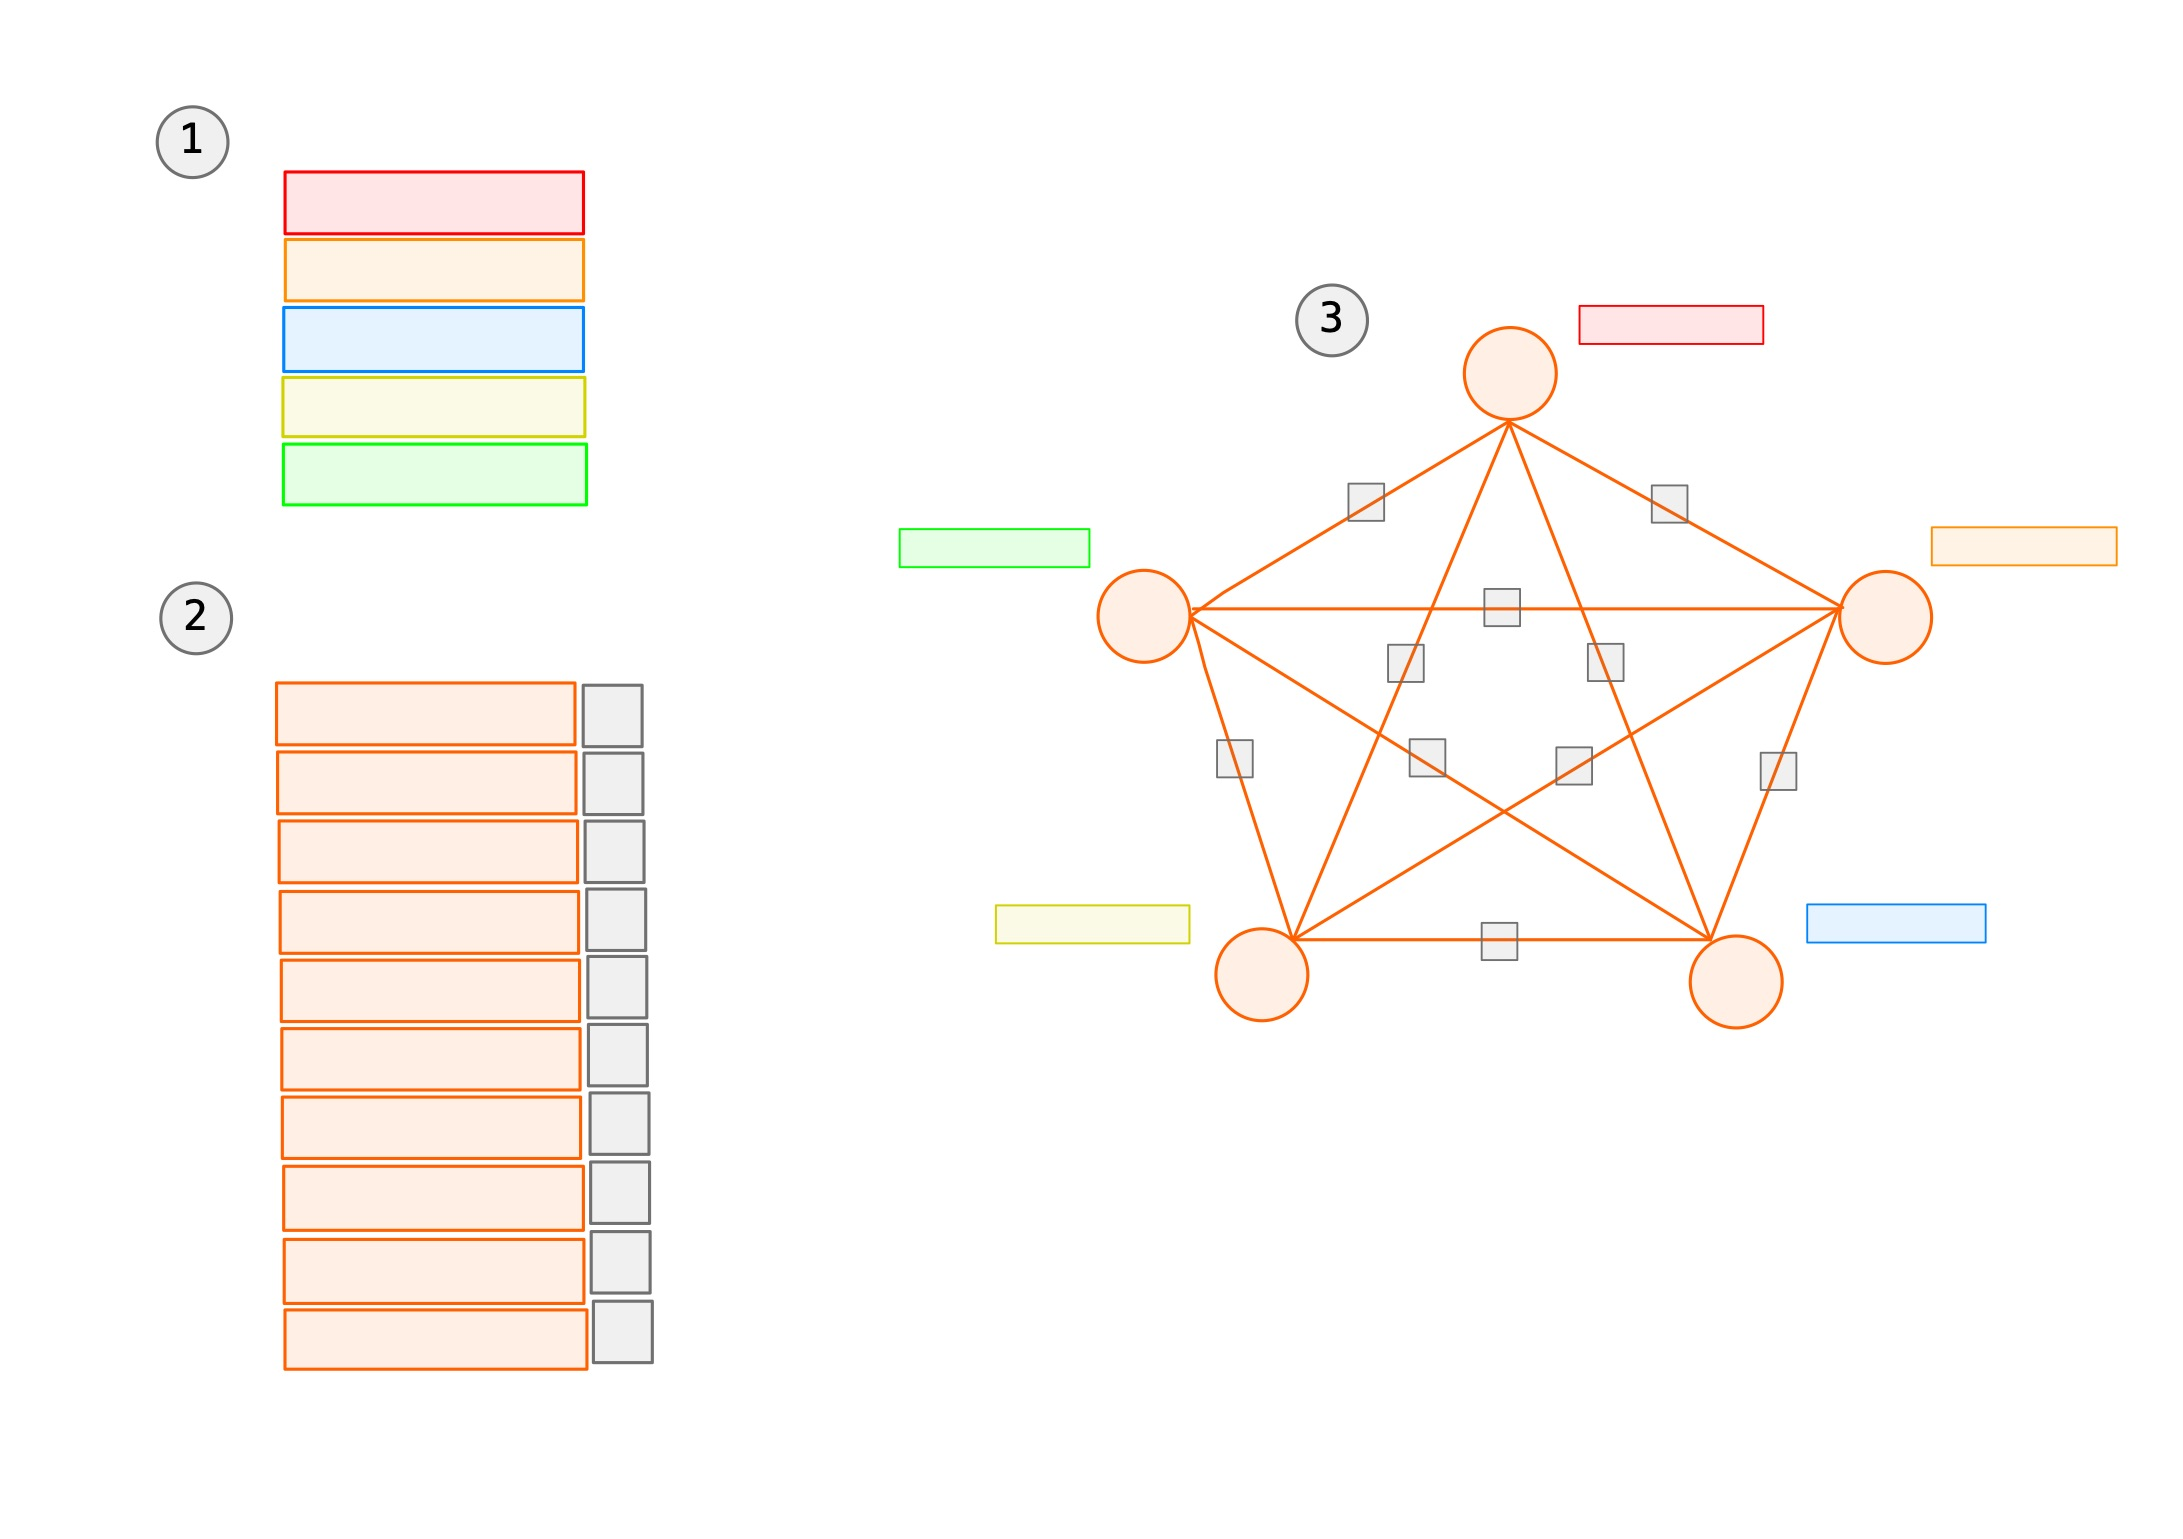
\includegraphics[width=\textwidth]{gcn-data.jpg}
  \caption{Overview of GCN dataset creation procedure. \textbf{(1)} an
    example of the main dataset with 5 hits. \textbf{(2)} the
    corresponding modified MLP dataset created. Although the dataset
    will contain $n^{2}-n = 25$ rows, only the unique rows (10 in this
    example) are shown in the illustration for simplicity.
    \textbf{(3)} The graph representation is created where rows of (1)
    become the node embeddings and the label column of (2) become the
    edge weights.}
  \label{fig:gcn-data}
\end{figure}

A modified MLP dataset (see \ref{sec:mlp-data-prep}) with a shape of
\texttt{$(n^{2}-n, 5)$} is created such that each hit is paired with
all other hits except itself. The label column from this dataset is
then used as the edge weights of the graph. Edges between event nodes
from the same event thus are assigned a weight of 1 and all other
edges are assigned a weight of 0.

Since the main dataset and the pattern matrix dataset are highly
skewed, naturally the GCN dataset is also skewed with majority of the
nodes being noise. Similar strategy as used in the creation of the
pattern matrix training set (see \ref{sec:mlp-data-prep}) is used. The
training set is a graph with approximately 1000 nodes equally
distributed amongst the classes. The skewed nature of the data is
maintained in the testing set. The model is evaluated with 3 test sets
each with varying levels of examples of event nodes. In practise, the
pipeline will observe timeslices with no to very few events thus the
performance of the model on test set 1 and 2 should be given
importance. The various test sets and their distribution are
summarized in Table \ref{gcn-test-dist}.

\begin{table}[htb]
  \centering
  \caption{Distribution of GCN testing datasets.}
  \begin{tabular}{lrrr}
    & Total examples & Positive examples & Negative examples \\
    \textbf{TS1} & 1000-1500 & -- & 1000-1500 \\
    \textbf{TS2} & 1000-1500 & 10-20 & 990-1480 \\
    \textbf{TS3} & 1000-1500 & 200-250 & 800-1250 \\
  \end{tabular}
  \label{tab:gcn-test-dst}
\end{table}

\section{Model Description and Evaluation}
\label{sec:gcn-model-desc-eval}

The model is expected to classify nodes of an unseen graph as event or
noise nodes. Since causally related nodes are connected with edges
carrying a high weight, the model is expected to group them together
thus resulting in a final graph with separate clusters of causally
related nodes and noise nodes.

\begin{table}[htb]
  \centering
  \begin{tabular}{lr}
    \hline
    Loss & BCELoss \\
    Optimizer & Adam with learning rate of $0.001$ \\
    Hidden Activation & ReLu \\
    Output Activation & Sigmoid \\
    \hline
  \end{tabular}
  \caption{GCN Model Parameter Summary.}
  \label{tab:gcn-model-param}
\end{table}

The parameters of the model are summarized in Table
\ref{tab:gcn-model-param}, the rational for selecting the parameters
being the same as that of the pattern matrix model (see
\ref{sec:mlp-model-desc}) since both models perform binary
classification. The difference comes from the model architecture which
is summarized in Table \ref{tab:gcn-model-arch}. The GCN model
comprises of an input layer, two graph convolusional layers and an
output layer. The network is fully connected with 4 neurons in the
input layer, 16 in both graph convolusional layers and 1 neuron in the
output layer. A dropout layer is added between the two Gconv layers to
prevent overfitting \ref{srivastava14dropout}.

\begin{table}
  \caption{GCN model architecture summary.}
  \begin{tabular}{lrrrr}
    \hline
    Layer position & Type & Activation & In features & Out features \\
    \hline
    1 & GConv & ReLU & 4 & 16 \\
    2 & dropout & -- & -- \\
    3 & GConv & RelU & 16 & 2 \\
    4 & Linear & Sigmoid & 2 & 1 \\
    \hline
  \end{tabular}
  \label{tab:gcn-model-arch}
\end{table}

Evaluation metrics used for evaluating the MLP model are used to
evaluate the GCD model as well (see Section \ref{sec:mlp-model-eval})
since the GCN dataset is also highly skewed in nature.

\section{Results}
\label{sec:gcd-disc}

\begin{figure}[htb]
  \centering
  \begin{minipage}{0.49\textwidth}
    \centering
    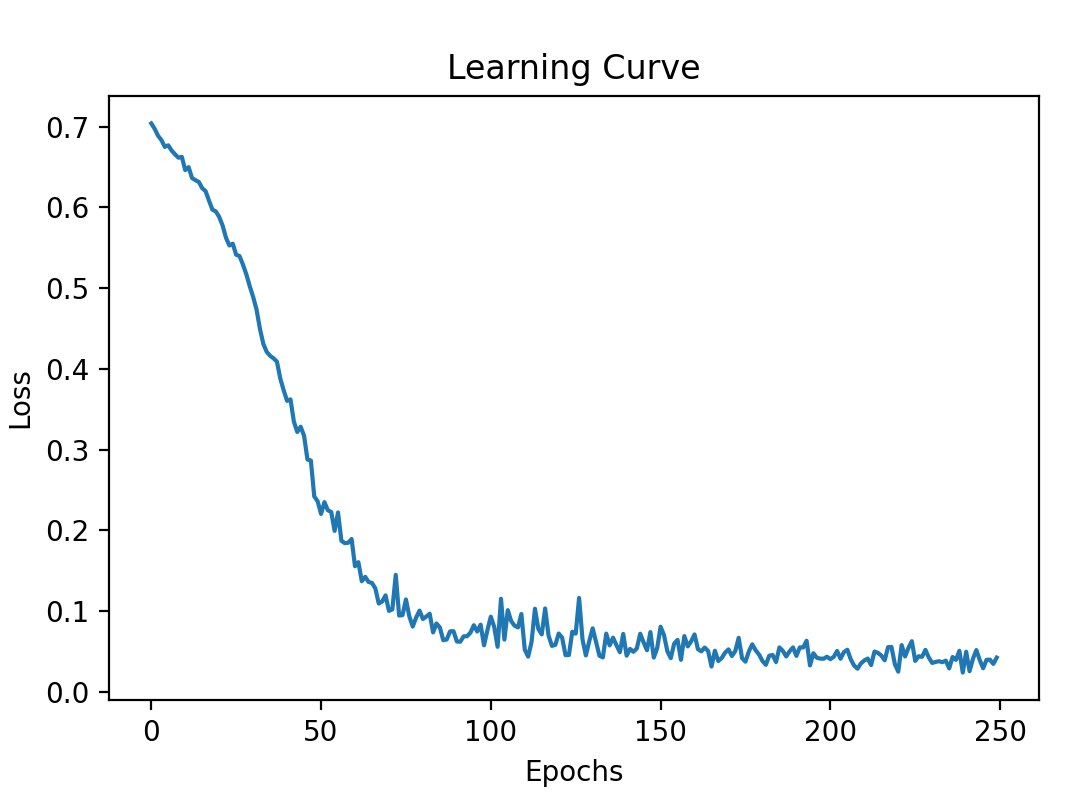
\includegraphics[width=\linewidth]{gcd-learning.png}
    \caption{Learning Curve for GCN with Naive Edge Weights.}
  \end{minipage}
  \begin{minipage}{0.49\textwidth}
    \centering
    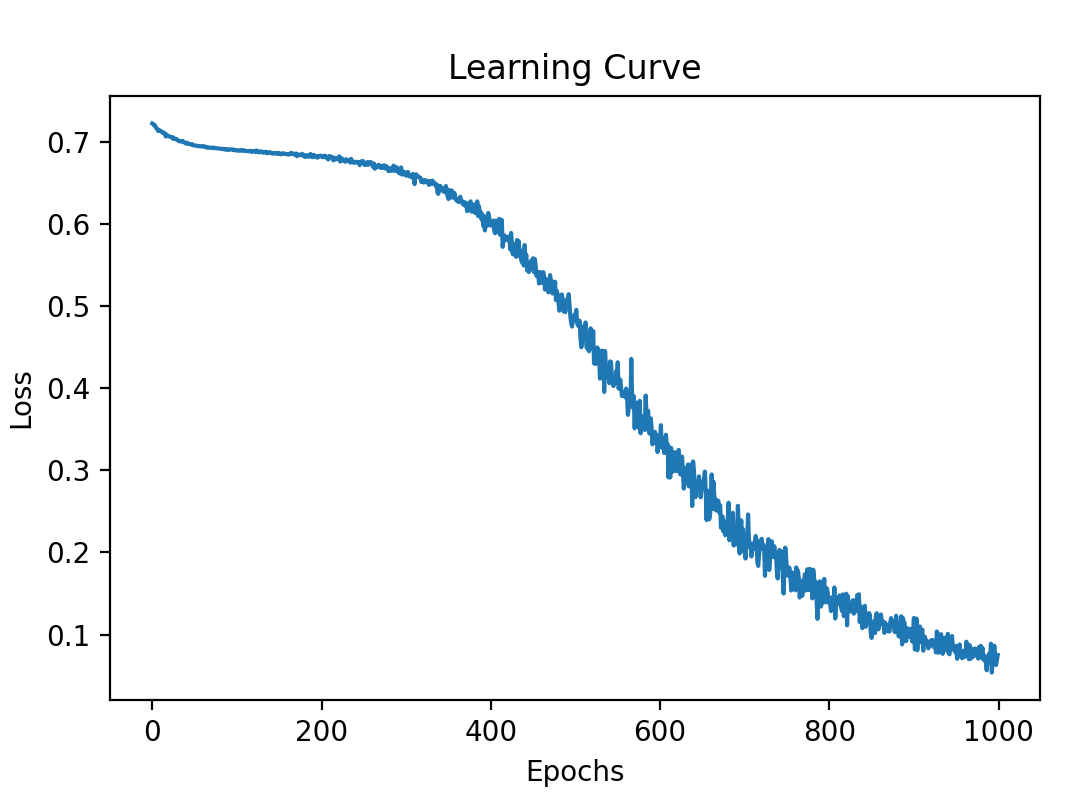
\includegraphics[width=\linewidth]{gcd-adv-learning.png}
    \caption{Learning Curve for GCN with Advanced Edge Weights.}
  \end{minipage}
  \caption{Learning Curves for GCN Training Datasets.}
  \label{fig:gcn-learning}
\end{figure}

\begin{table}[htb]
  \begin{tabular}{lrrrrrrr}
    \hline
    & Accuracy & Precision & Recall & F1 & F2 & ROCAUC & PRAUC \\
    \hline
    \multicolumn{8}{c}{Primitive edge weights} \\
    \hline
    TS1 & TODO & -- & -- & -- & -- & -- & -- \\
    TS2 & 0.58 & 0.04 & 1.00 & 0.08 & 0.18 & 0.87 & 0.06 \\
    TS3 & 0.67 & 0.40 & 1.00 & 0.57 & 0.77 & 0.81 & 0.36 \\
    \hline
    \multicolumn{8}{c}{Advanced edge weights} \\
    \hline
    TS1 & TODO & -- & -- & -- & -- & -- & -- \\
    TS2 & 1.00 & 1.00 & 1.00 & 1.00 & 1.00 & 1.00 & 1.00 \\
    TS3 & 1.00 & 1.00 & 1.00 & 1.00 & 1.00 & 1.00 & 1.00 \\    
  \end{tabular}
  \caption{Summary of GCN performance across test sets.}
  \label{tab:gcn-results}
\end{table}

A good fit is achieved by the model on both training datasets as seen
in Figure \ref{fig:gcn-learning} although a slower learning rate and
longer training epochs were necessary for the later. In addition to
the model's performance on the various test sets as summarized by Table
\ref{tab:gcn-results}, the node embedding of the training and testing
graphs are also inspected using t-SNE \ref{maaten2008visualizing}.
Figure \ref{fig:gcn-train-tsne} shows the node embedding of the
training datasets before and after training. It is interesting to note
that the model is indeed able to learn as clusters of similar nodes
are noticed after training, with the model being able to cluster noise
nodes into larger and fewer communities when training using advanced
weights. Inspecting Figure \ref{fig:gcn-test-tsne} one can see the
model's ability to cluster similar nodes in the testing sets.

\begin{figure}[htb]
  \centering
  \begin{minipage}{0.49\textwidth}
    \centering
    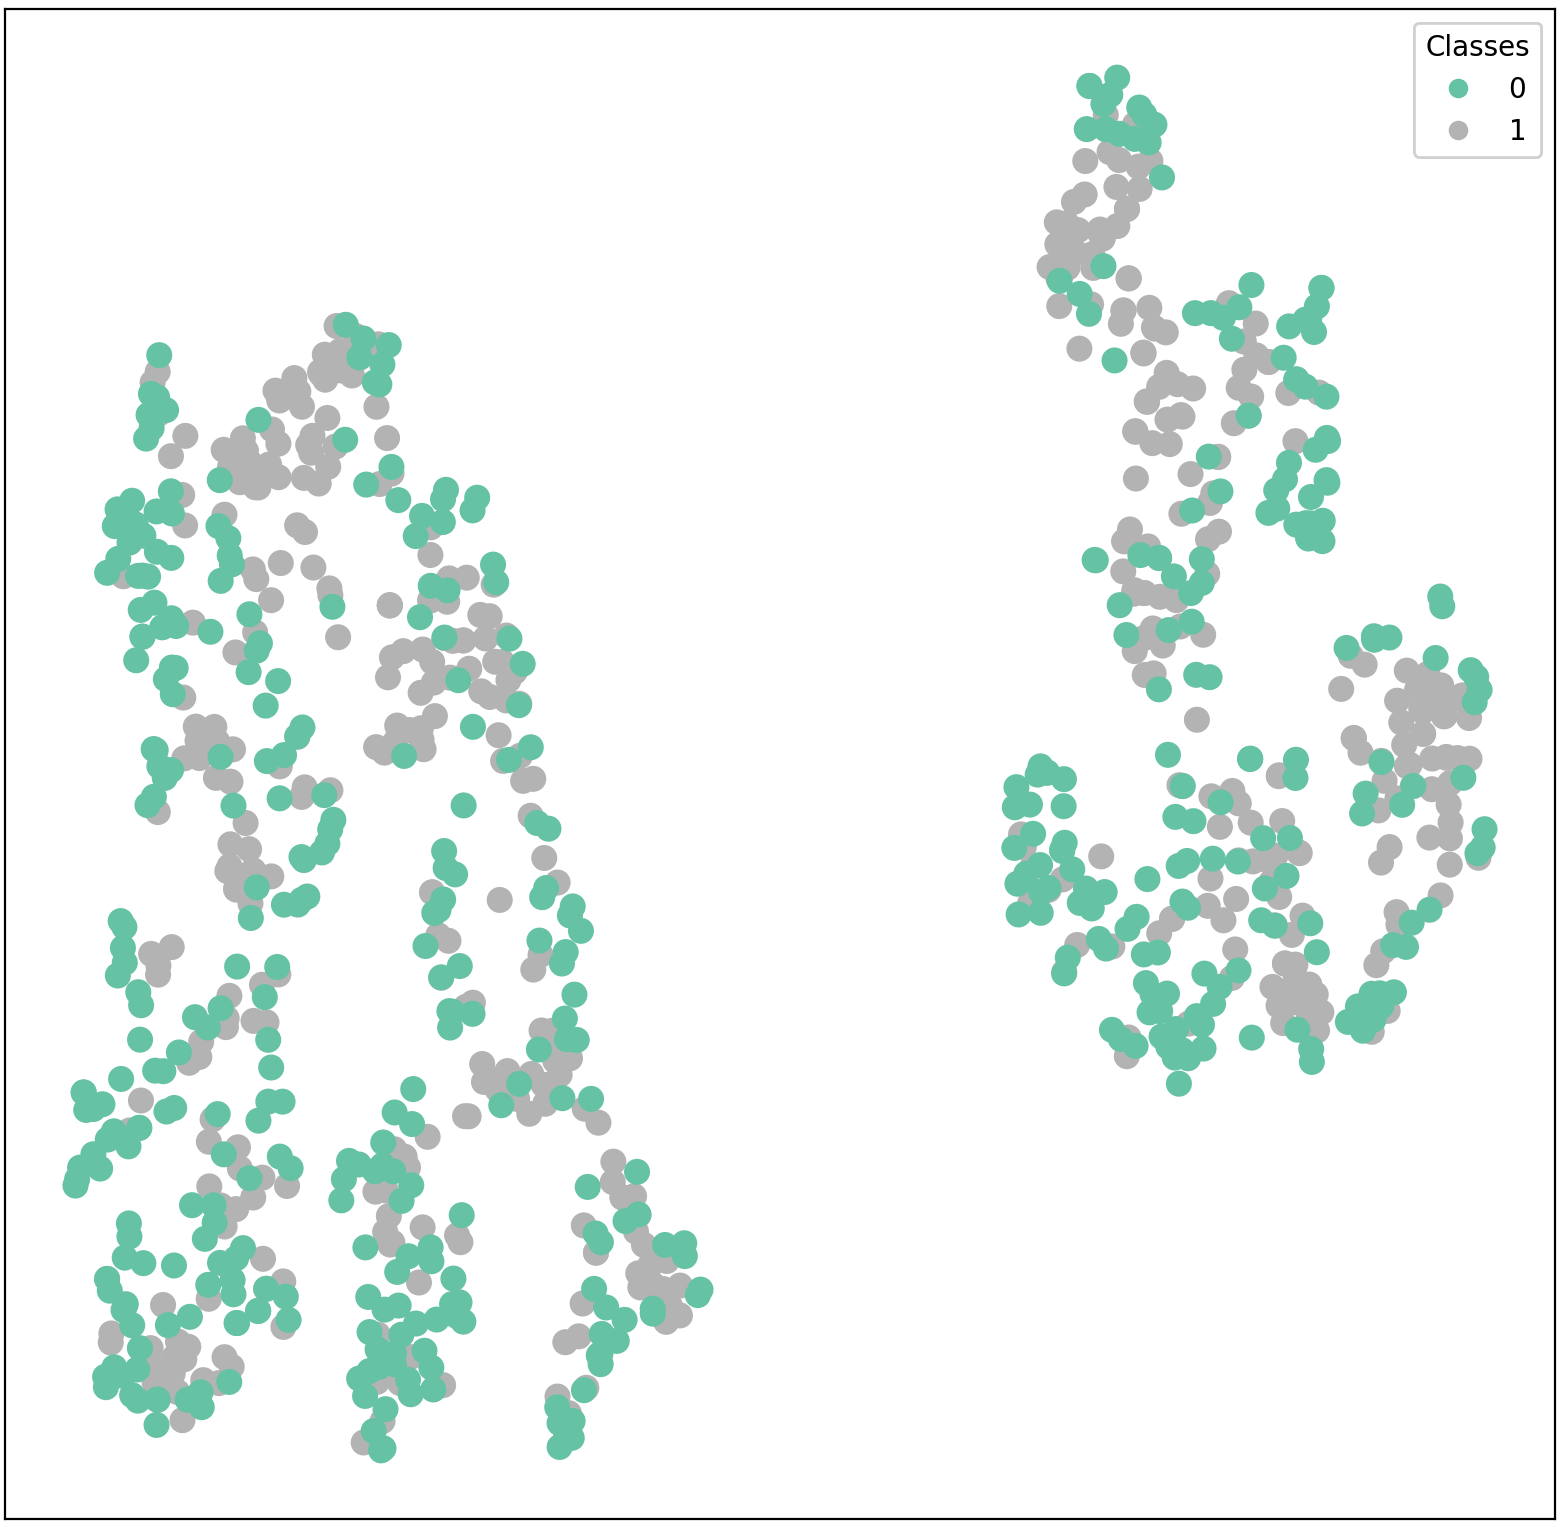
\includegraphics[width=\linewidth]{gcd-train-tsne.png}
    \caption{TSNE for training set (naive edge weights) before training.}
  \end{minipage}
  \begin{minipage}{0.49\textwidth}
    \centering
    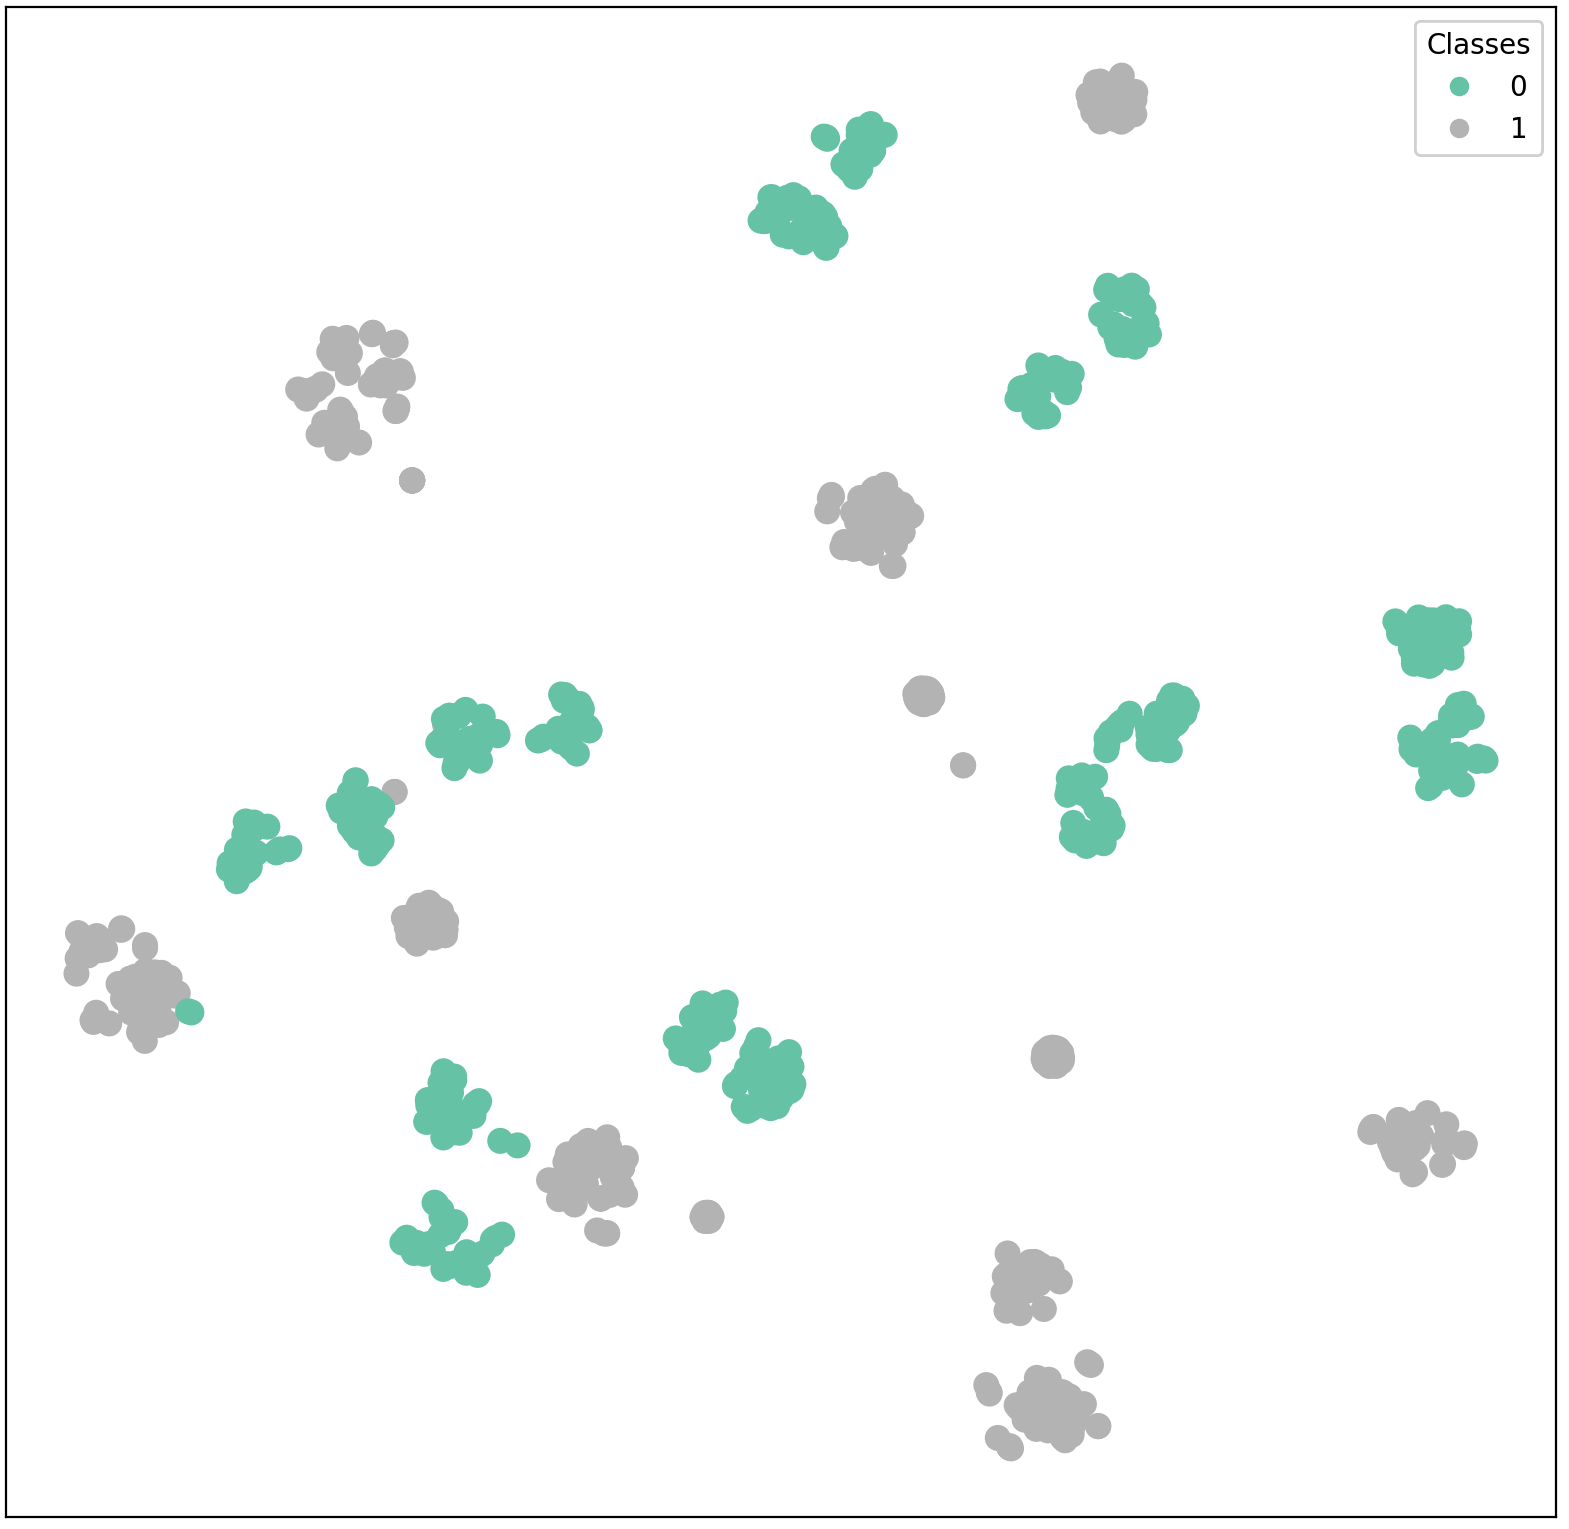
\includegraphics[width=\linewidth]{gcd-train-tsne-after.png}
    \caption{TSNE for training set (naive edge weights) after training.}
  \end{minipage}
  \begin{minipage}{0.49\textwidth}
    \centering
    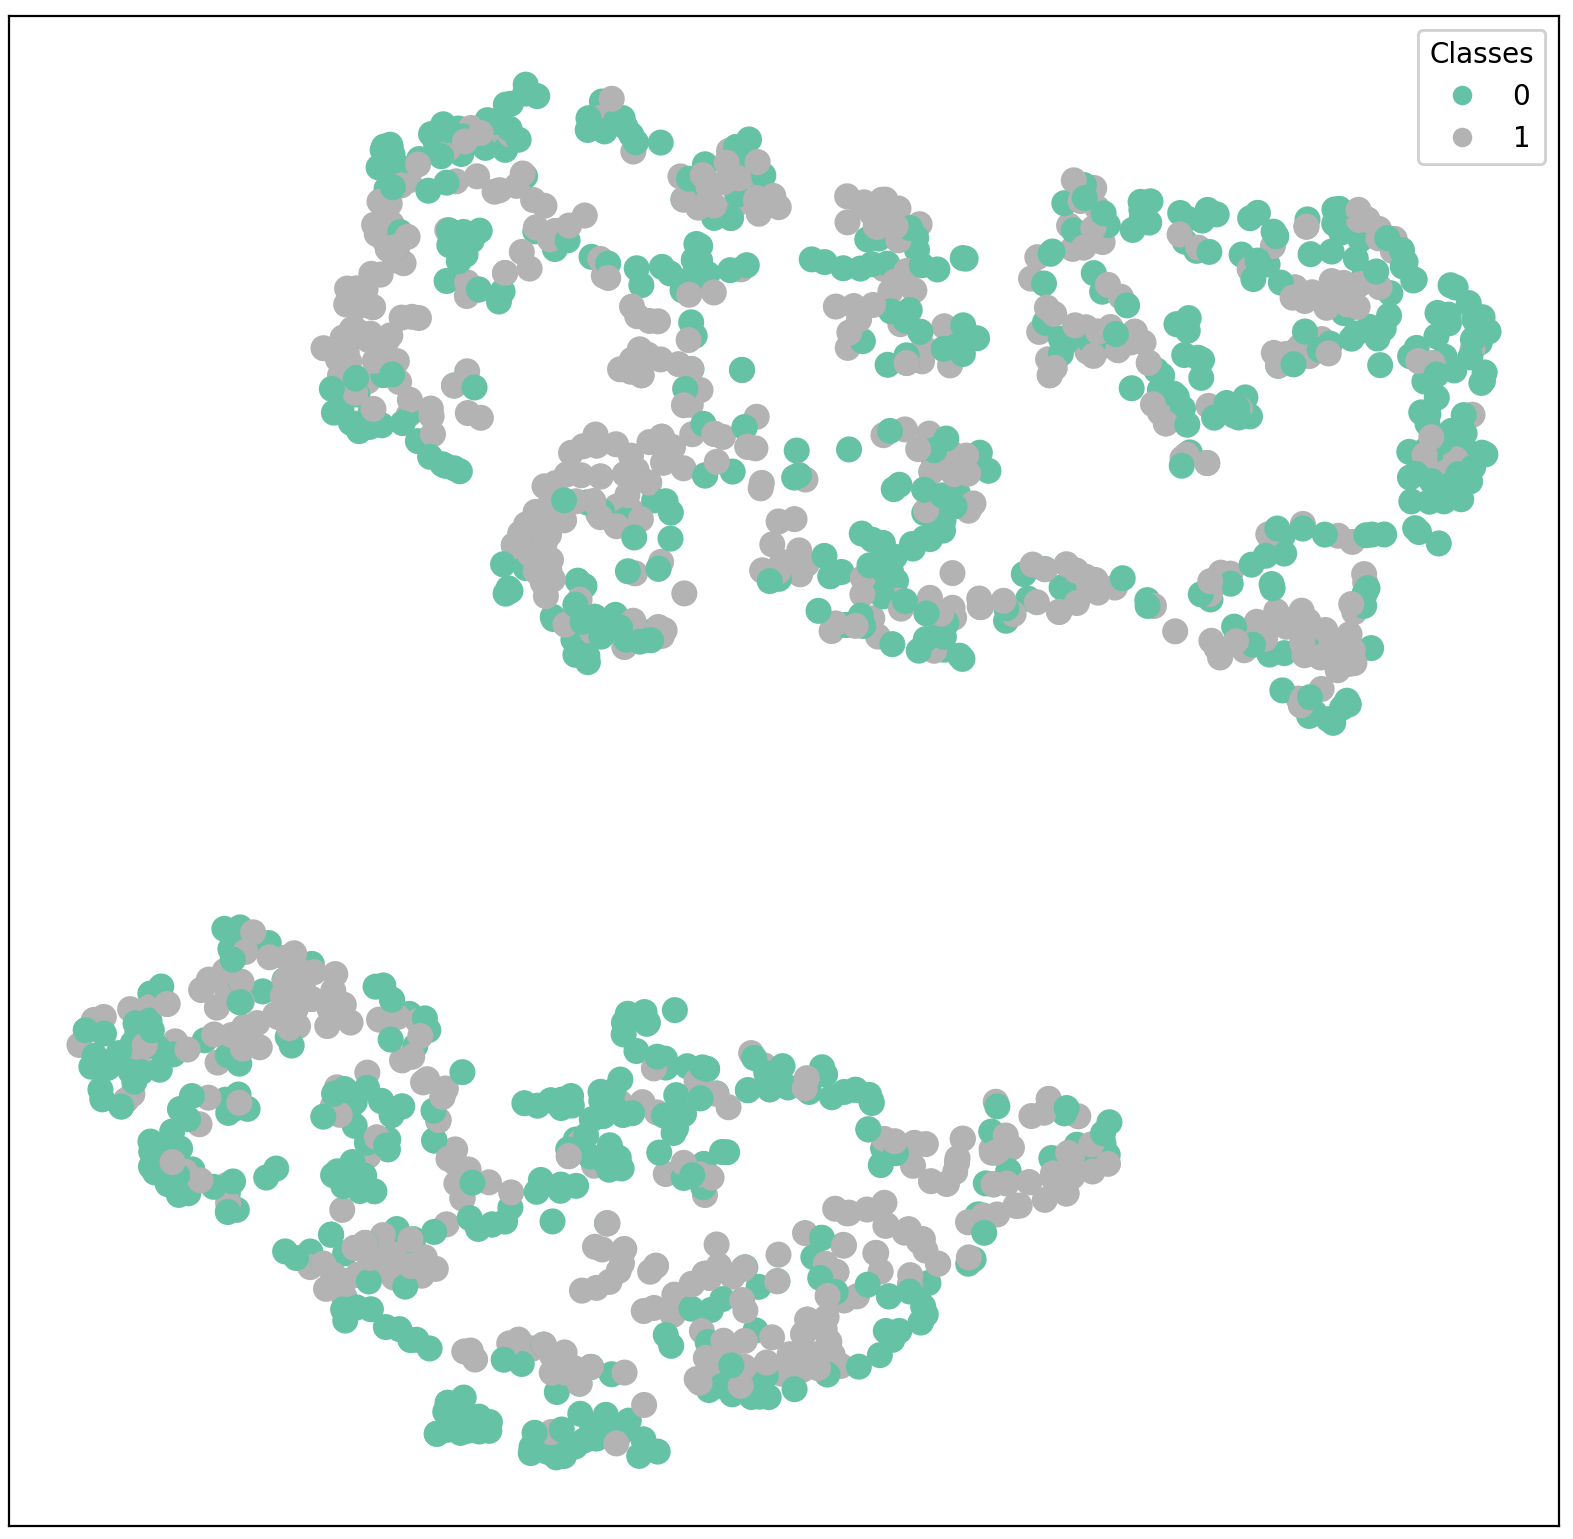
\includegraphics[width=\linewidth]{gcd-adv-train-tsne.png}
    \caption{TSNE for training set (advanced edge weights) before training.}
  \end{minipage}
  \begin{minipage}{0.49\textwidth}
    \centering
    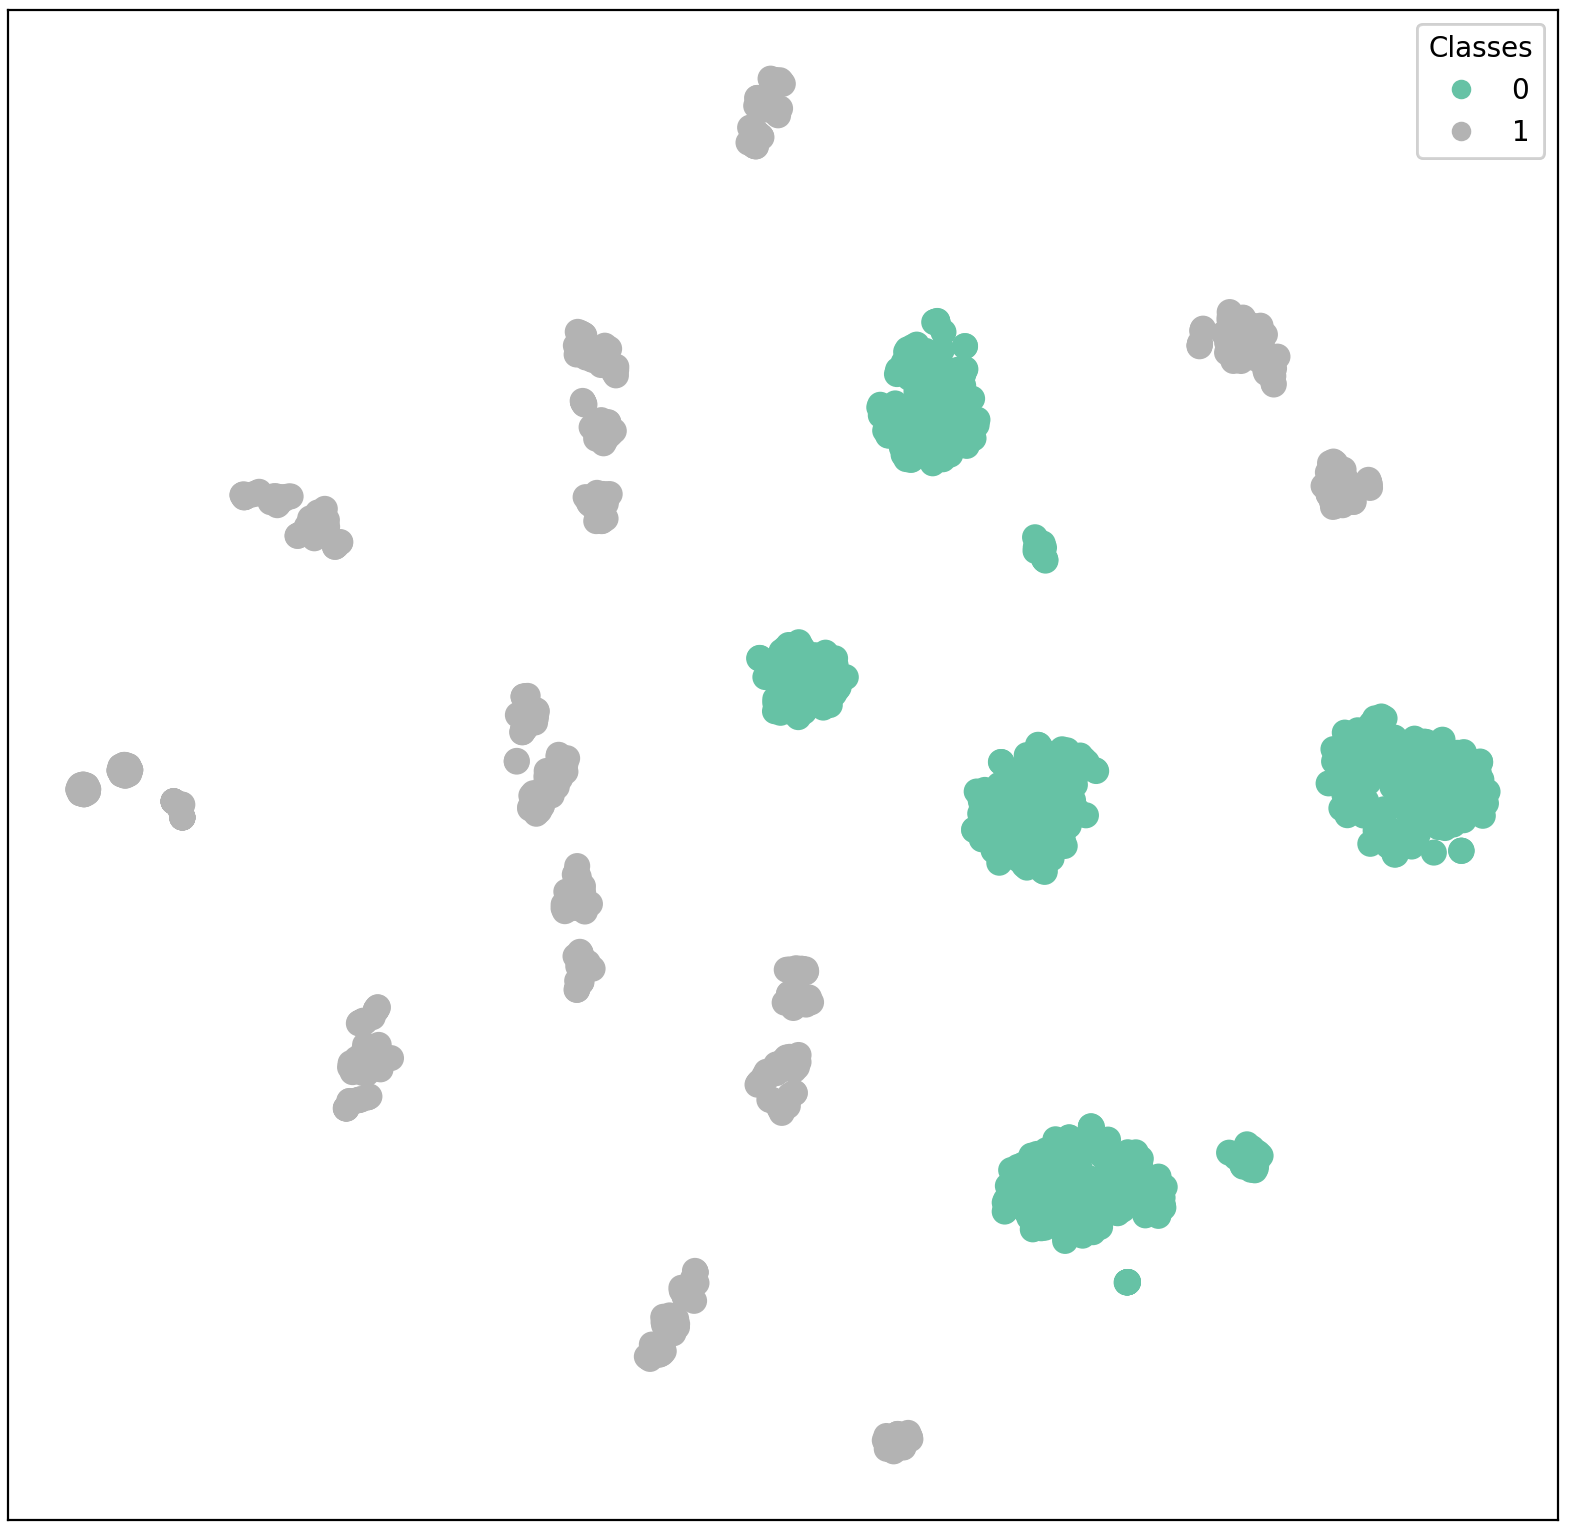
\includegraphics[width=\linewidth]{gcd-adv-train-tsne-after.png}
    \caption{TSNE for training set (advanced edge weights) after training.}
  \end{minipage}
  \caption{TSNE for GCN Training Datasets.}
  \label{fig:gcn-train-tsne}
\end{figure}

Very scarce communities are observed when the model is trained using
naive edge weights. The model is clearly unable to form any
communities in TS1 and TS2 and is only able to cluster the event nodes
in TS3. It is evident that the model is unable to identify noise nodes
when trained using naive edge weights. In fact, it is biased to the
minority class as is seen in the Confusion Matrices depicted in Figure
\ref{gcn-cm}. The model is able to identify all event nodes in TS2 and
TS3 perfectly however has a high number of FPs. This indicates that
the presence of the high edge weights assigned to causally related
nodes greatly aids the model in identifying the event nodes. However,
since all other edges are assigned a weight of 0, the model does not
quite learn to identify the noise nodes.

\begin{figure}[htb]
  \centering
  \begin{minipage}{0.32\textwidth}
    \centering
    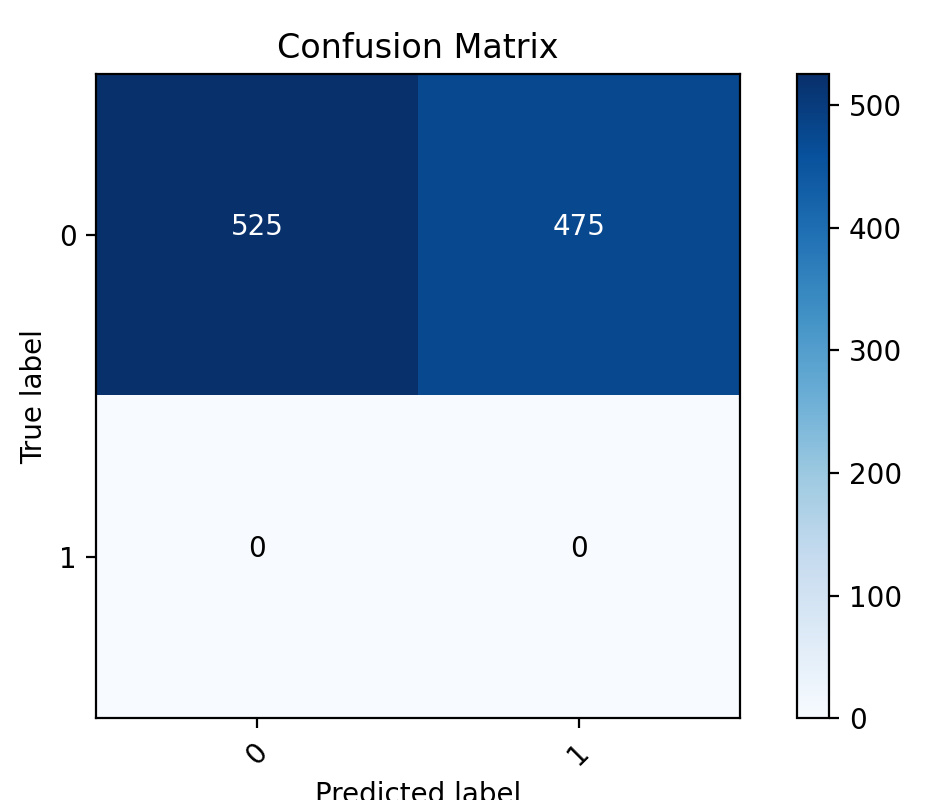
\includegraphics[width=\linewidth]{gcd-cm-no.png}
    \caption{CM for TS1 (naive edge weights).}
  \end{minipage}
  \begin{minipage}{0.32\textwidth}
    \centering
    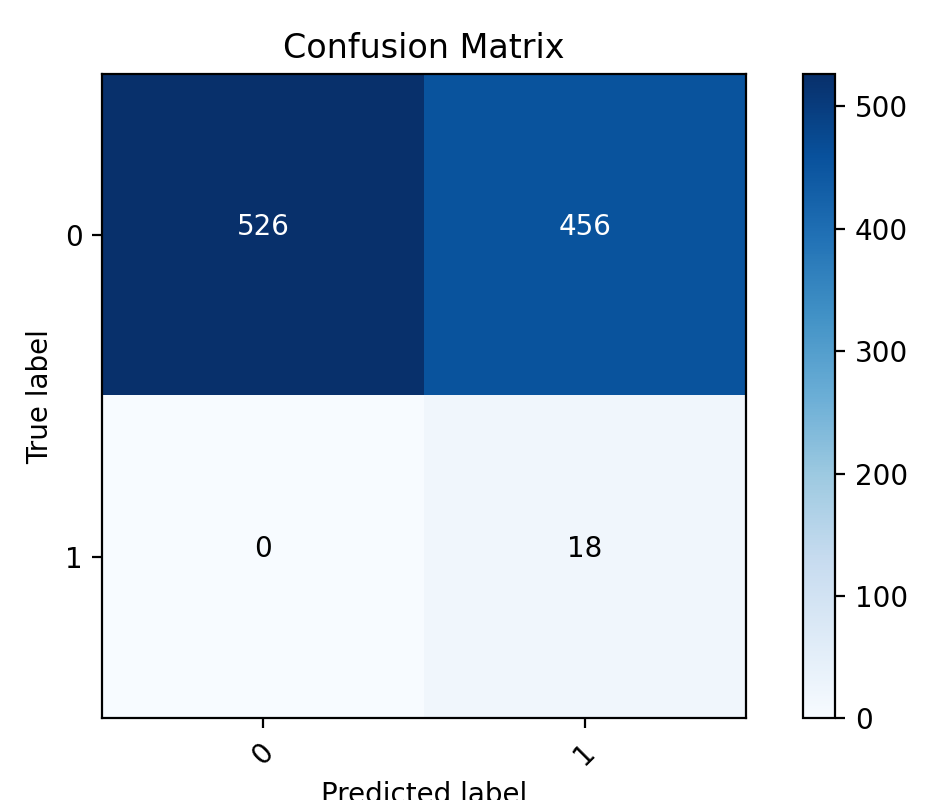
\includegraphics[width=\linewidth]{gcd-cm-medium.png}
    \caption{CM for TS2 (naive edge weights).}
  \end{minipage}
  \begin{minipage}{0.32\textwidth}
    \centering
    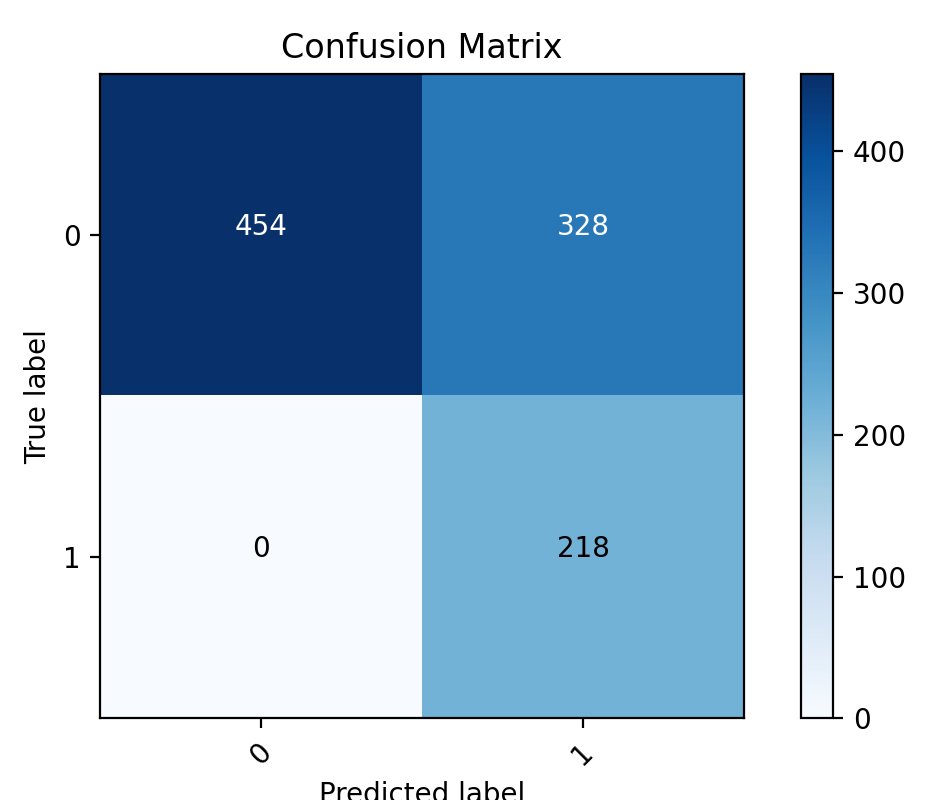
\includegraphics[width=\linewidth]{gcd-cm-high.png}
    \caption{CM for TS3 (naive edge weights).}
  \end{minipage}
  \begin{minipage}{0.32\textwidth}
    \centering
    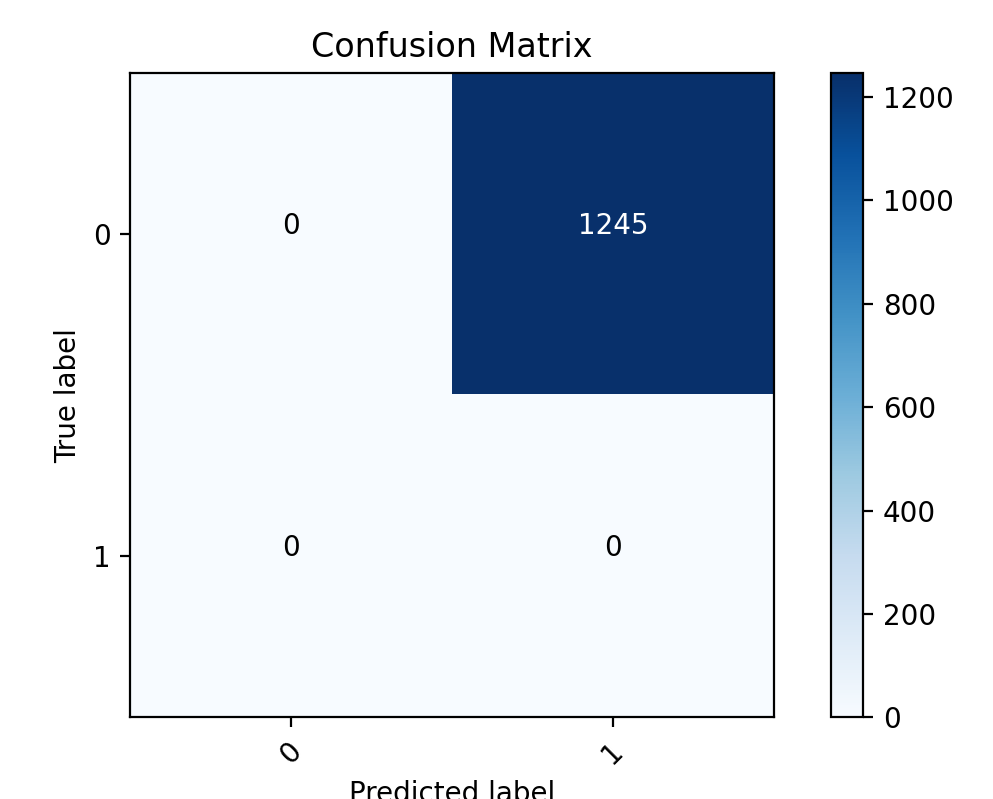
\includegraphics[width=\linewidth]{gcd-adv-cm-no.png}
    \caption{CM for TS1 (advanced edge weights).}
  \end{minipage}
  \begin{minipage}{0.32\textwidth}
    \centering
    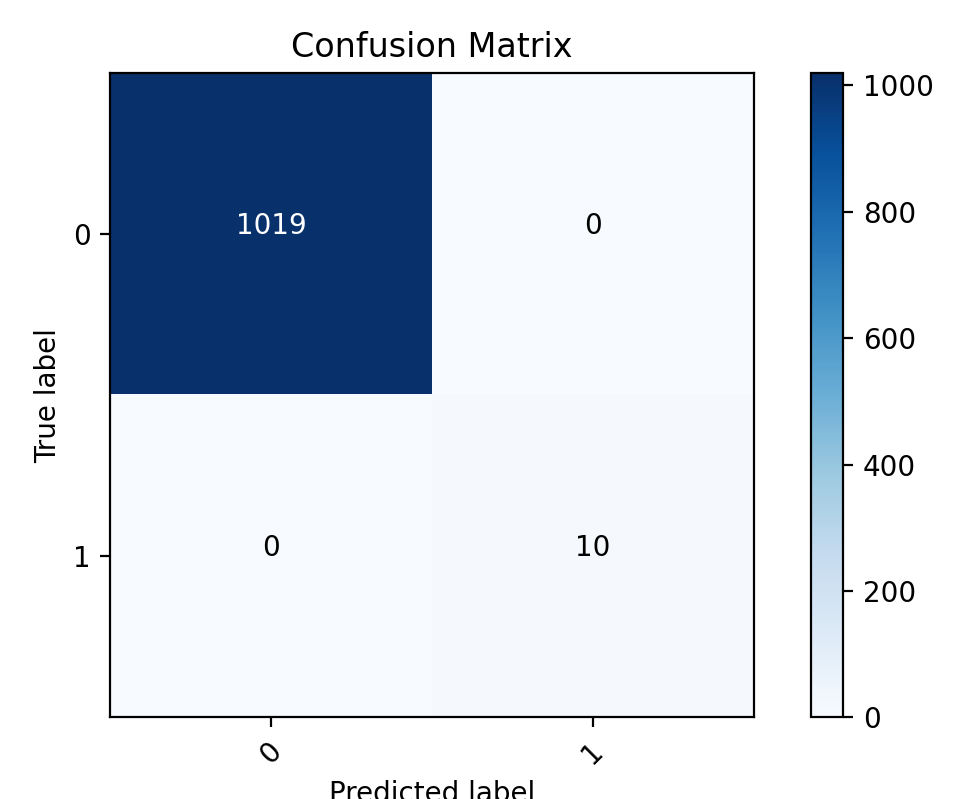
\includegraphics[width=\linewidth]{gcd-adv-cm-medium.png}
    \caption{CM for TS2 (advanced edge weights).}
  \end{minipage}
  \begin{minipage}{0.32\textwidth}
    \centering
    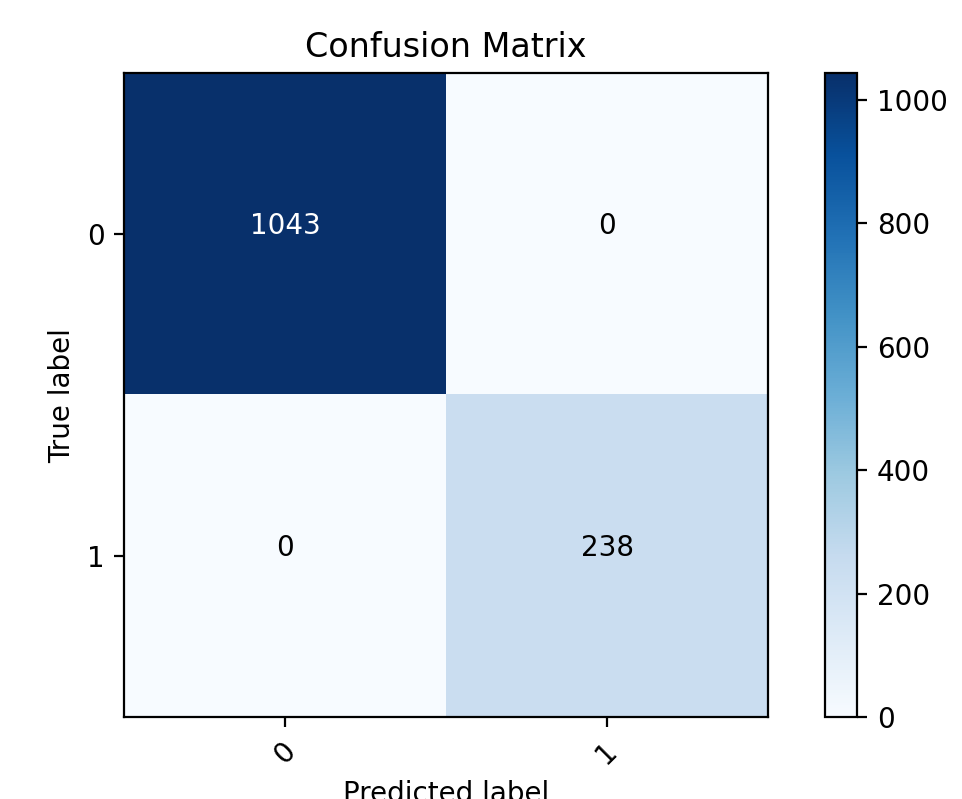
\includegraphics[width=\linewidth]{gcd-adv-cm-high.png}
    \caption{CM for TS3 (advanced edge weights).}
  \end{minipage}  
  \caption{CM for GCN Test Datasets.}
  \label{fig:gcn-cm}
\end{figure}

The performance of the model when training using the advanced edge
weights has a stark contrast with respect to the former. On initial
observation of Figure \ref{gcn-test-tsne} one finds that the model is
not able to correctly cluster similar nodes. However, closer
inspection of the Confusion Matrices (see Figure \ref{gcn-cm}) reveals
that although the model performs perfectly on TS2 and TS3, it has an
accuracy of zero on TS1 with all nodes being classified as FPs.

\begin{figure}[htb]
  \centering
  \begin{minipage}{0.32\textwidth}
    \centering
    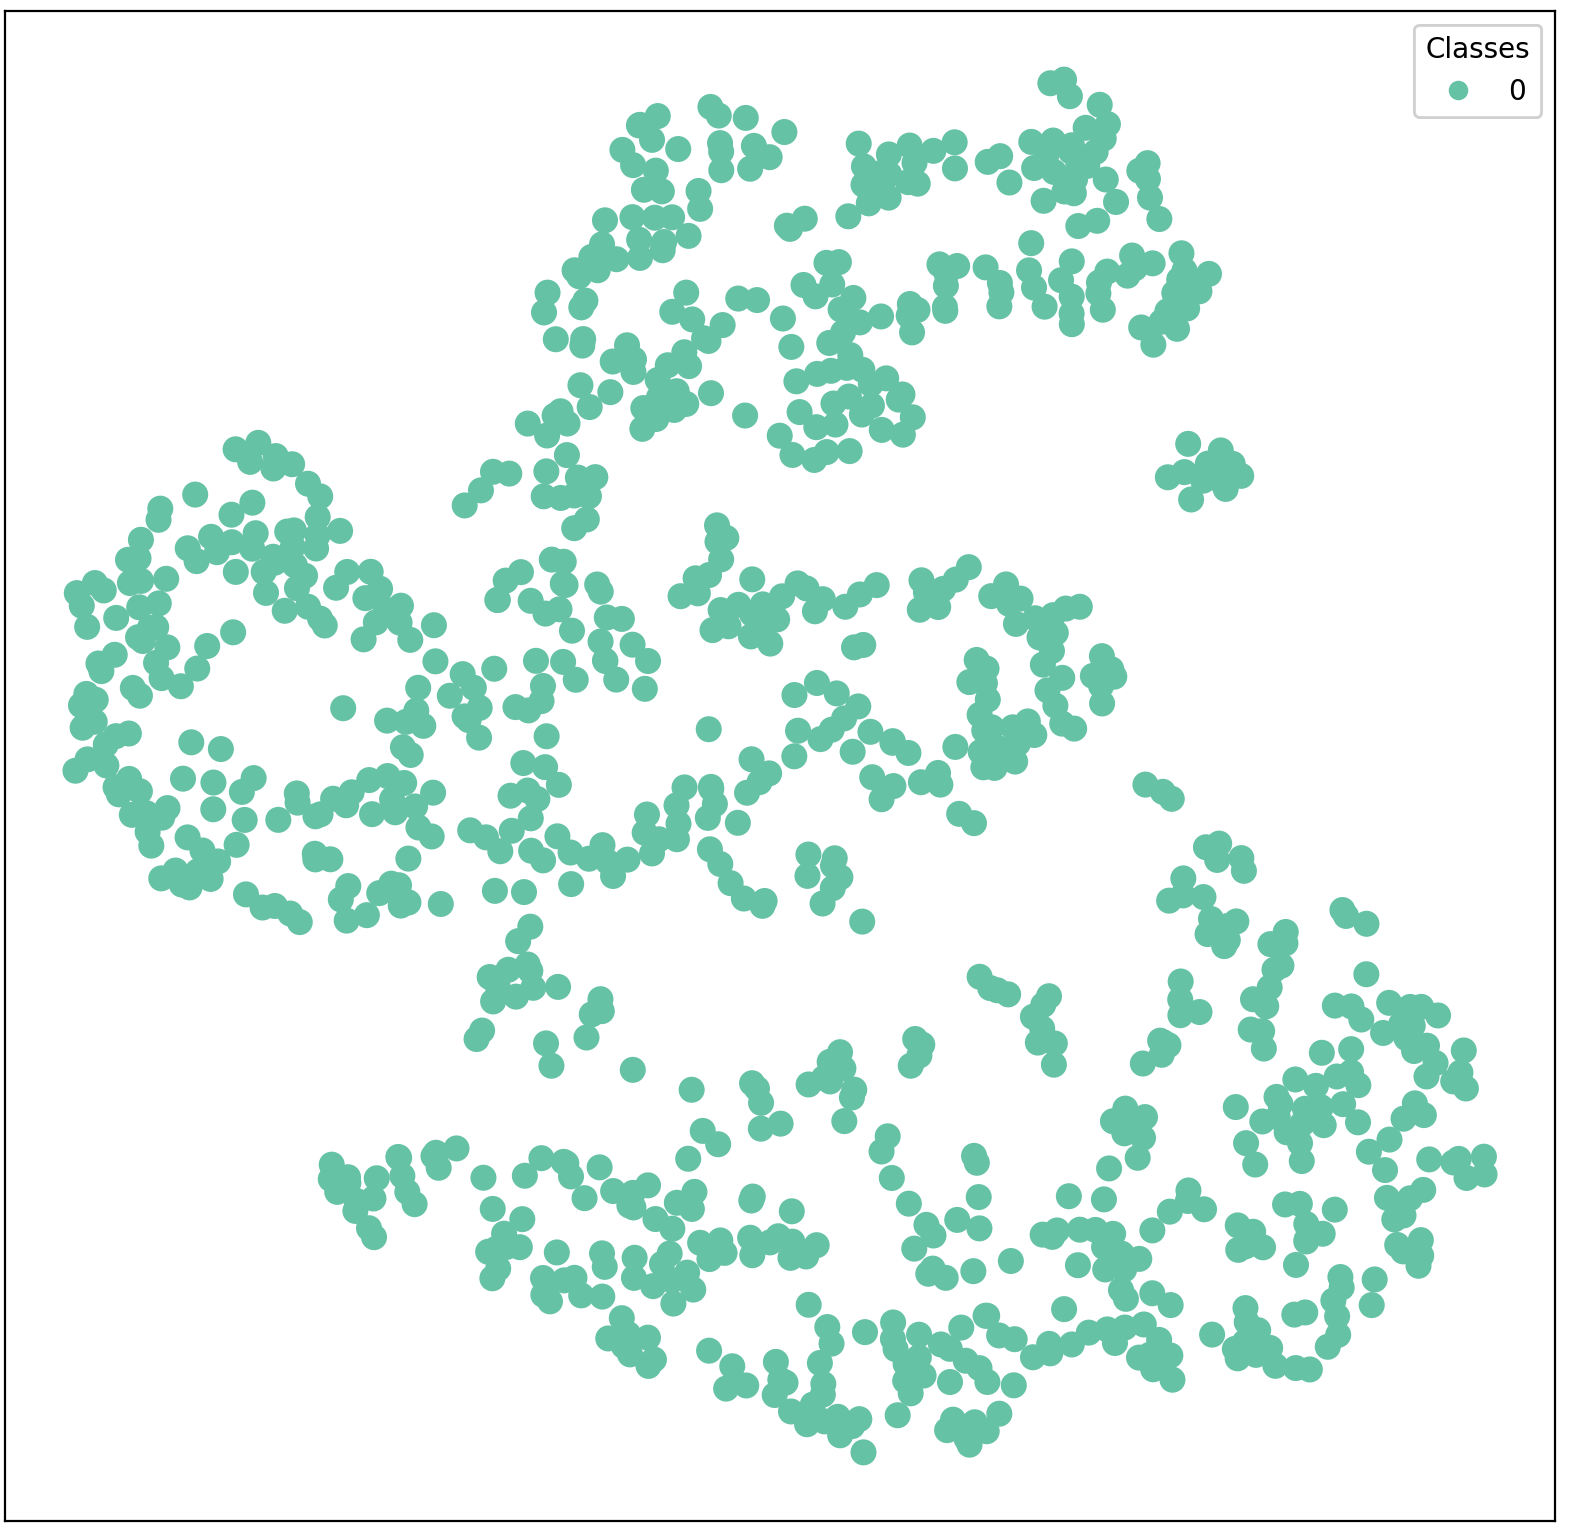
\includegraphics[width=\linewidth]{gcd-test-no-tsne.png}
    \caption{TSNE for TS1 (naive edge weights) before.}
  \end{minipage}
  \begin{minipage}{0.32\textwidth}
    \centering
    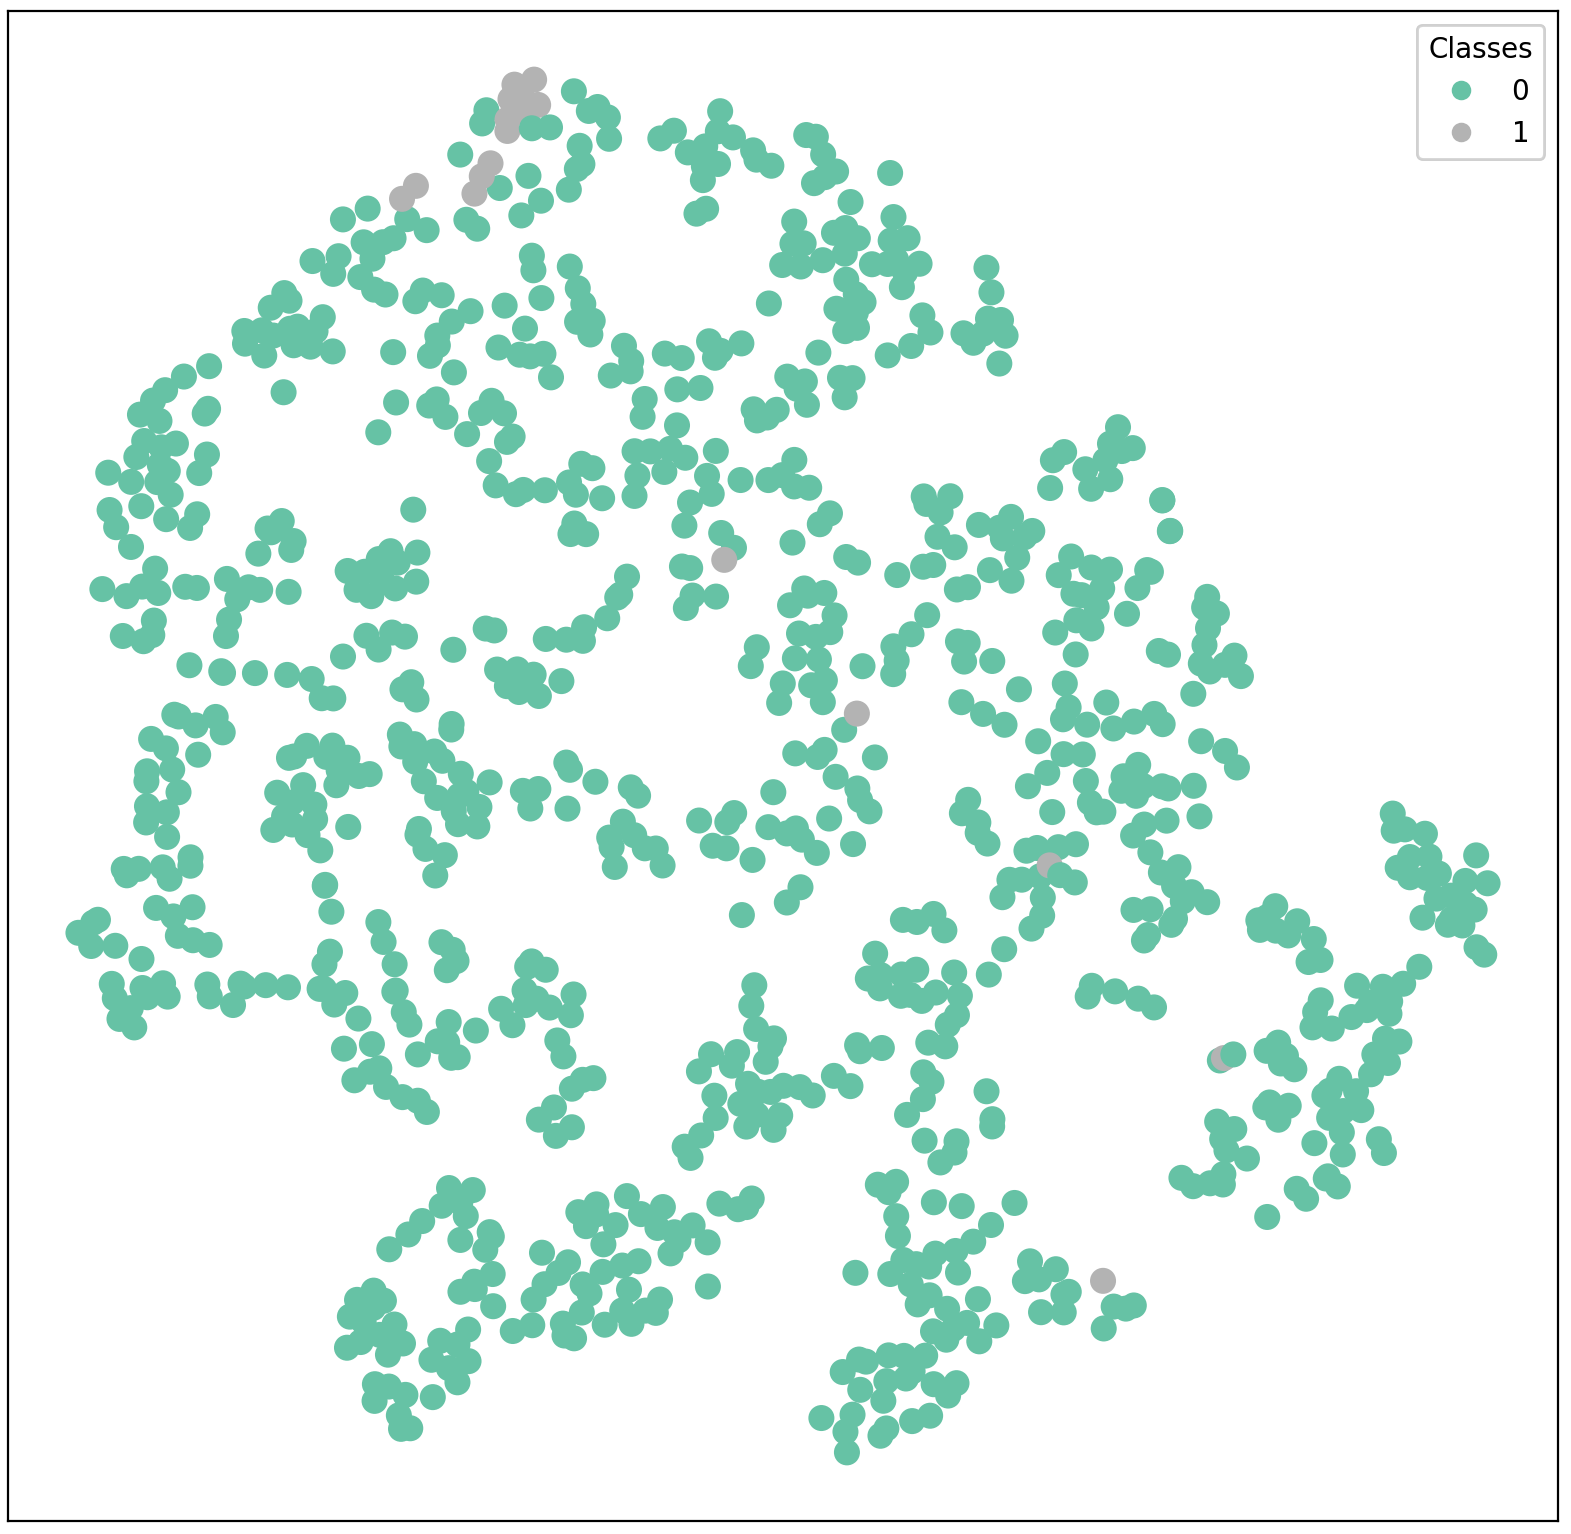
\includegraphics[width=\linewidth]{gcd-test-medium-tsne.png}
    \caption{TSNE for TS2 (naive edge weights) before.}
  \end{minipage}
  \begin{minipage}{0.32\textwidth}
    \centering
    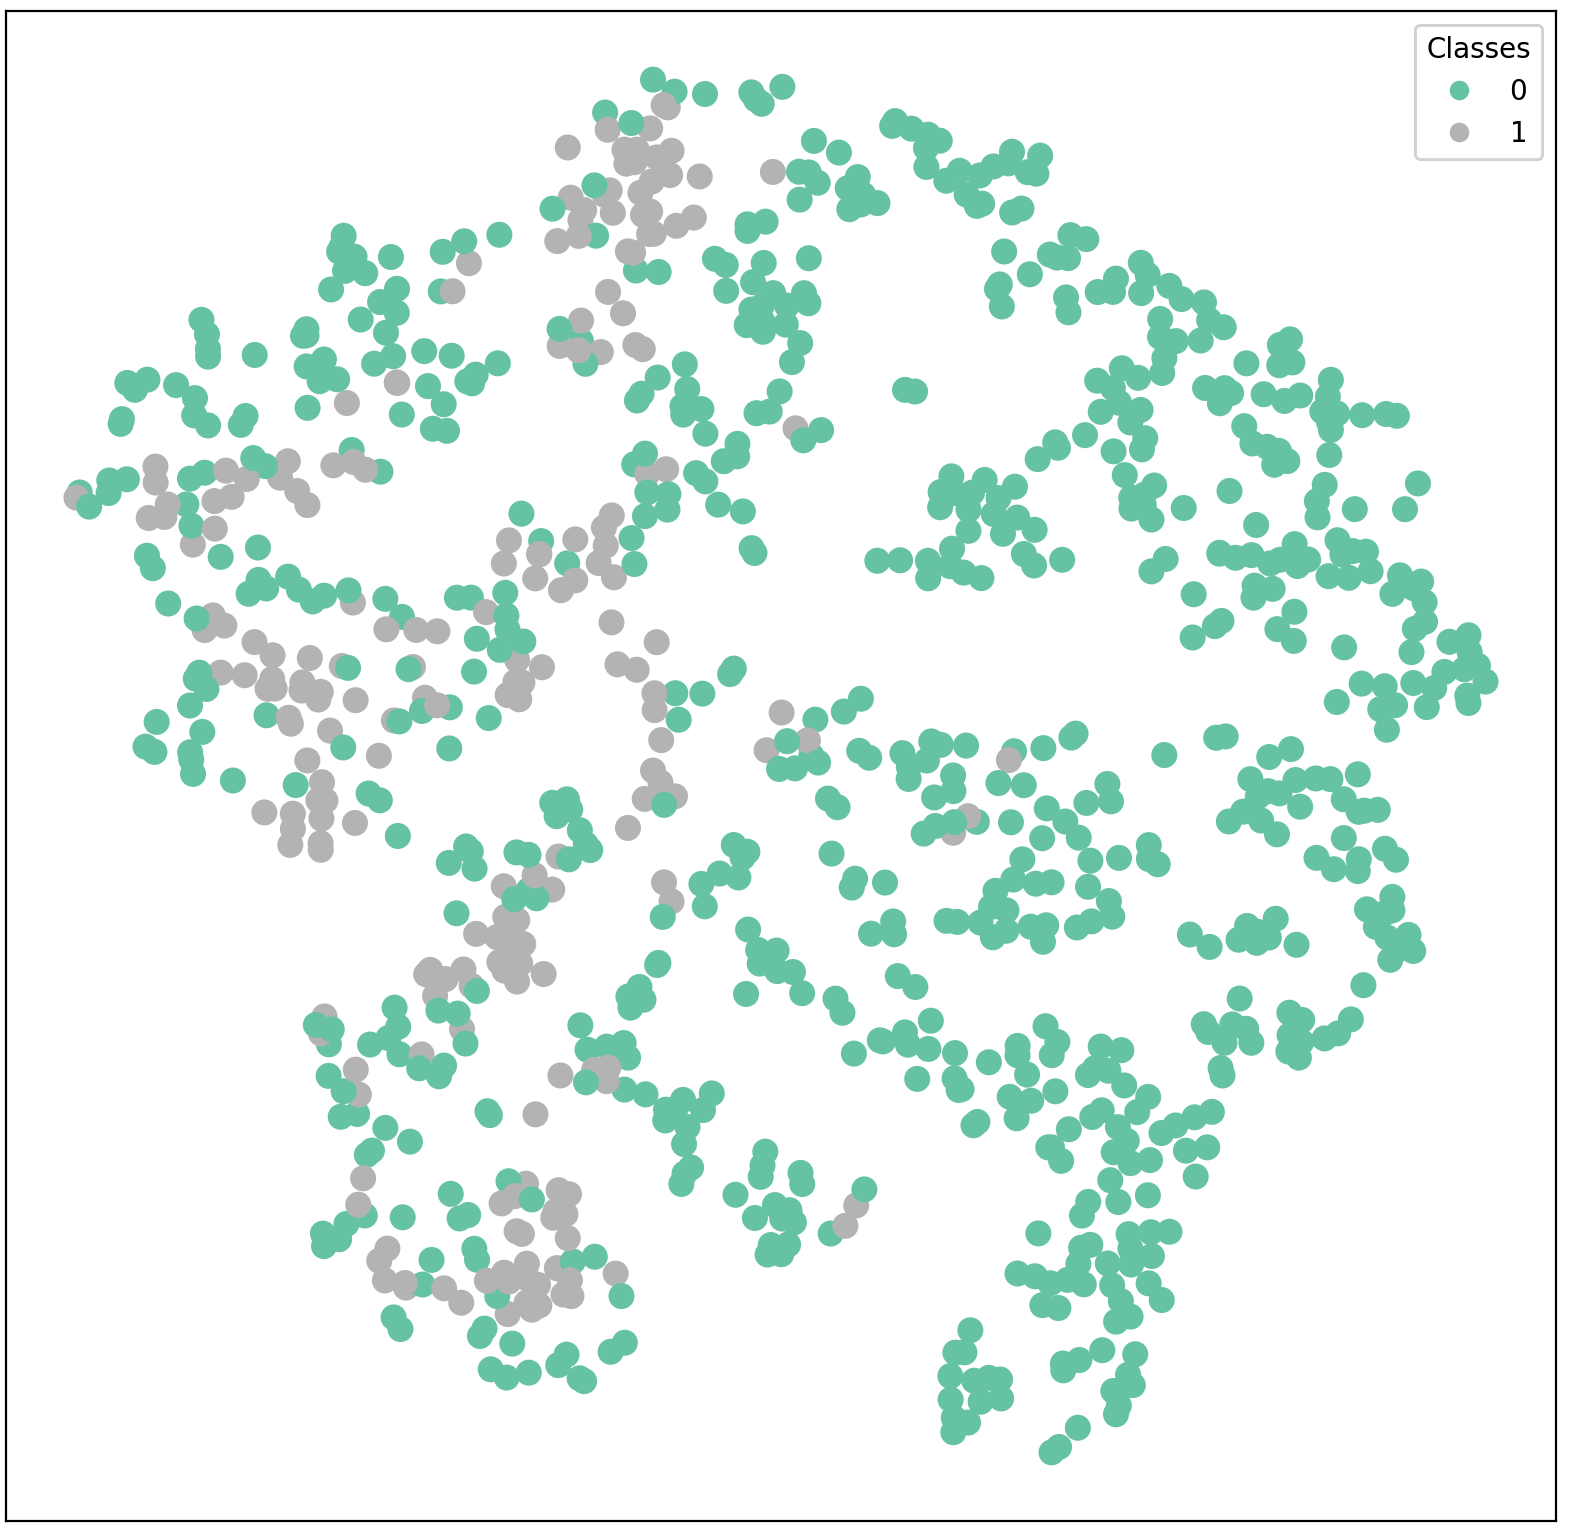
\includegraphics[width=\linewidth]{gcd-test-high-tsne.png}
    \caption{TSNE for TS3 (naive edge weights) before.}
  \end{minipage}
  \begin{minipage}{0.32\textwidth}
    \centering
    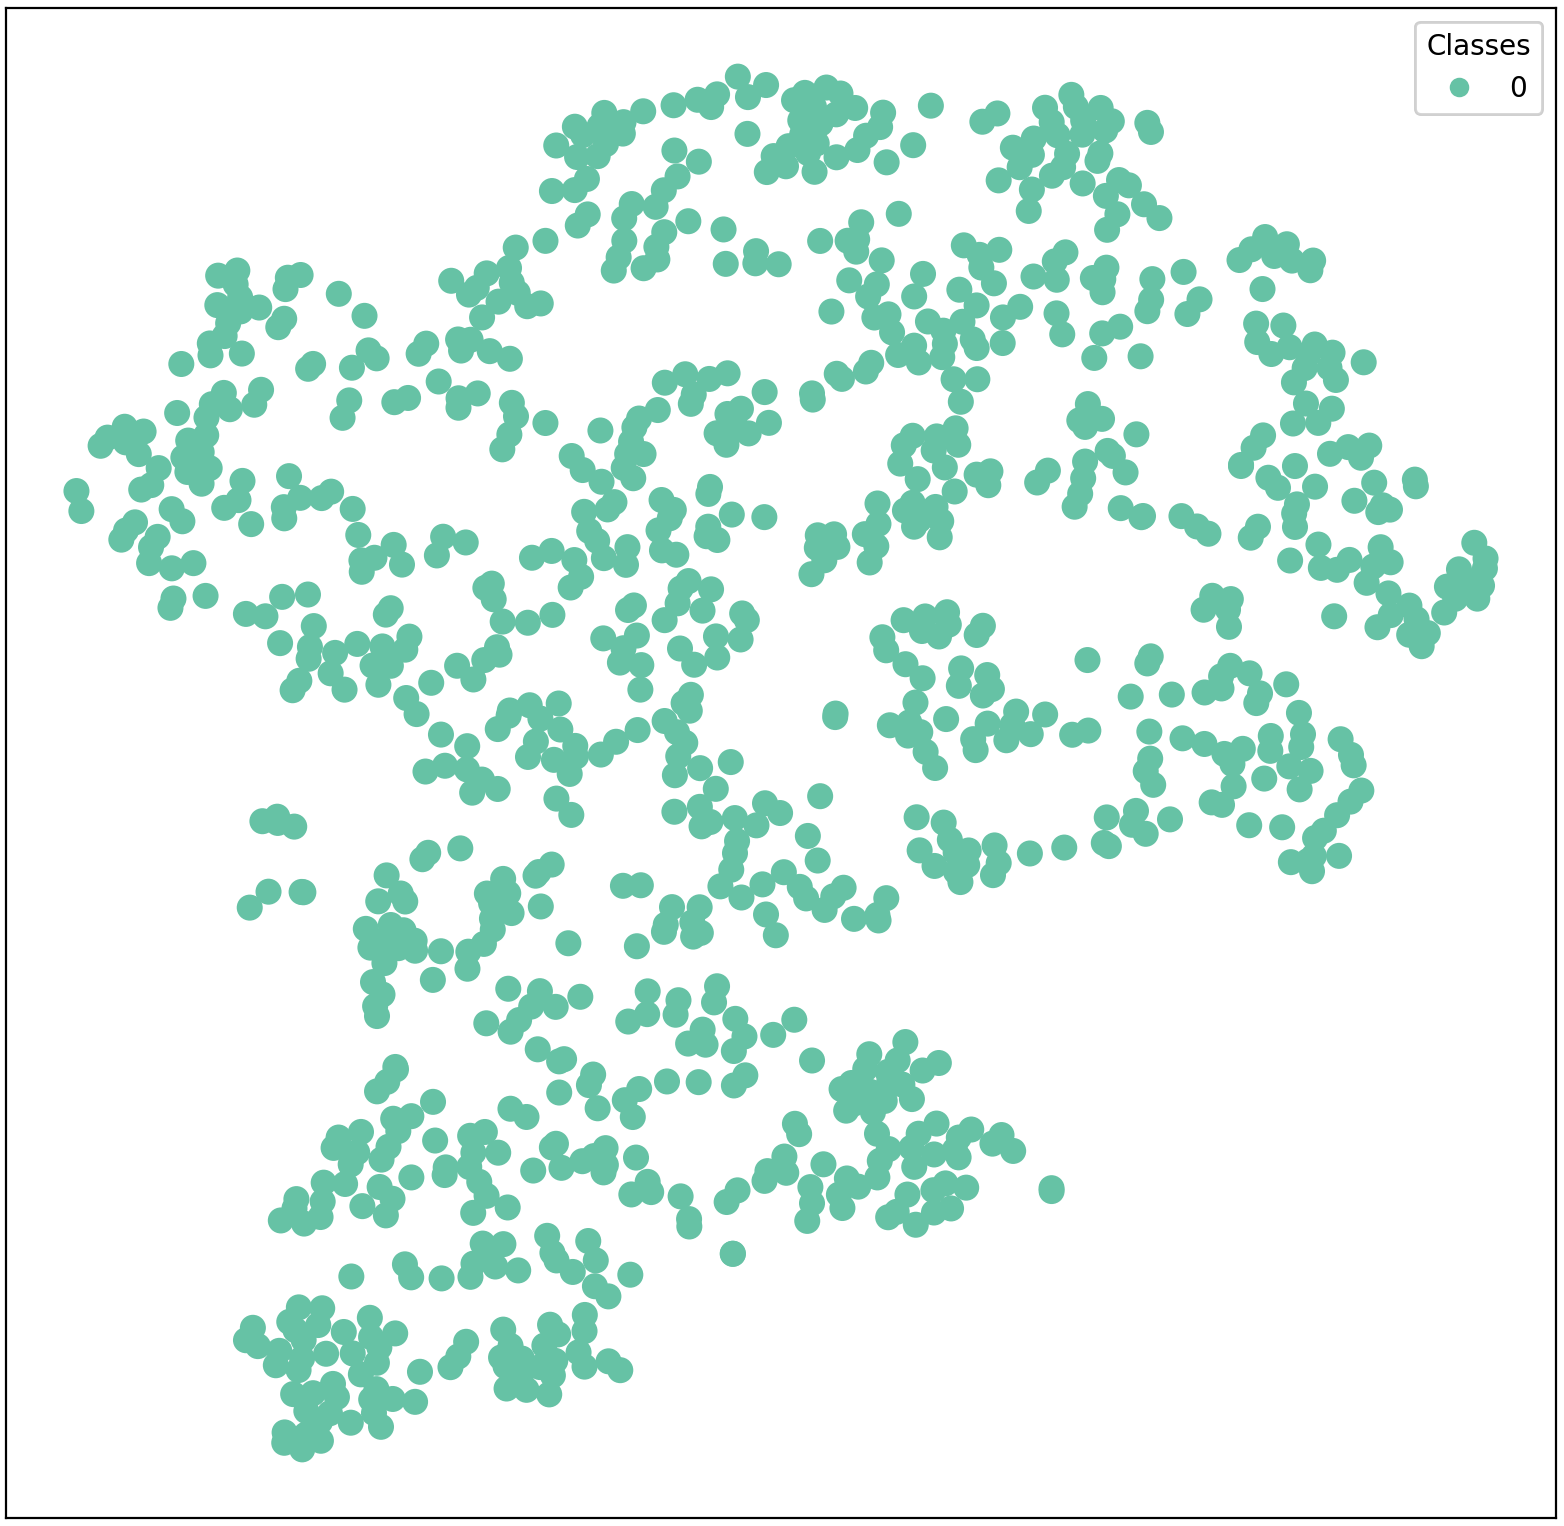
\includegraphics[width=\linewidth]{gcd-test-no-tsne-after.png}
    \caption{TSNE for TS1 (naive edge weights) after.}
  \end{minipage}
  \begin{minipage}{0.32\textwidth}
    \centering
    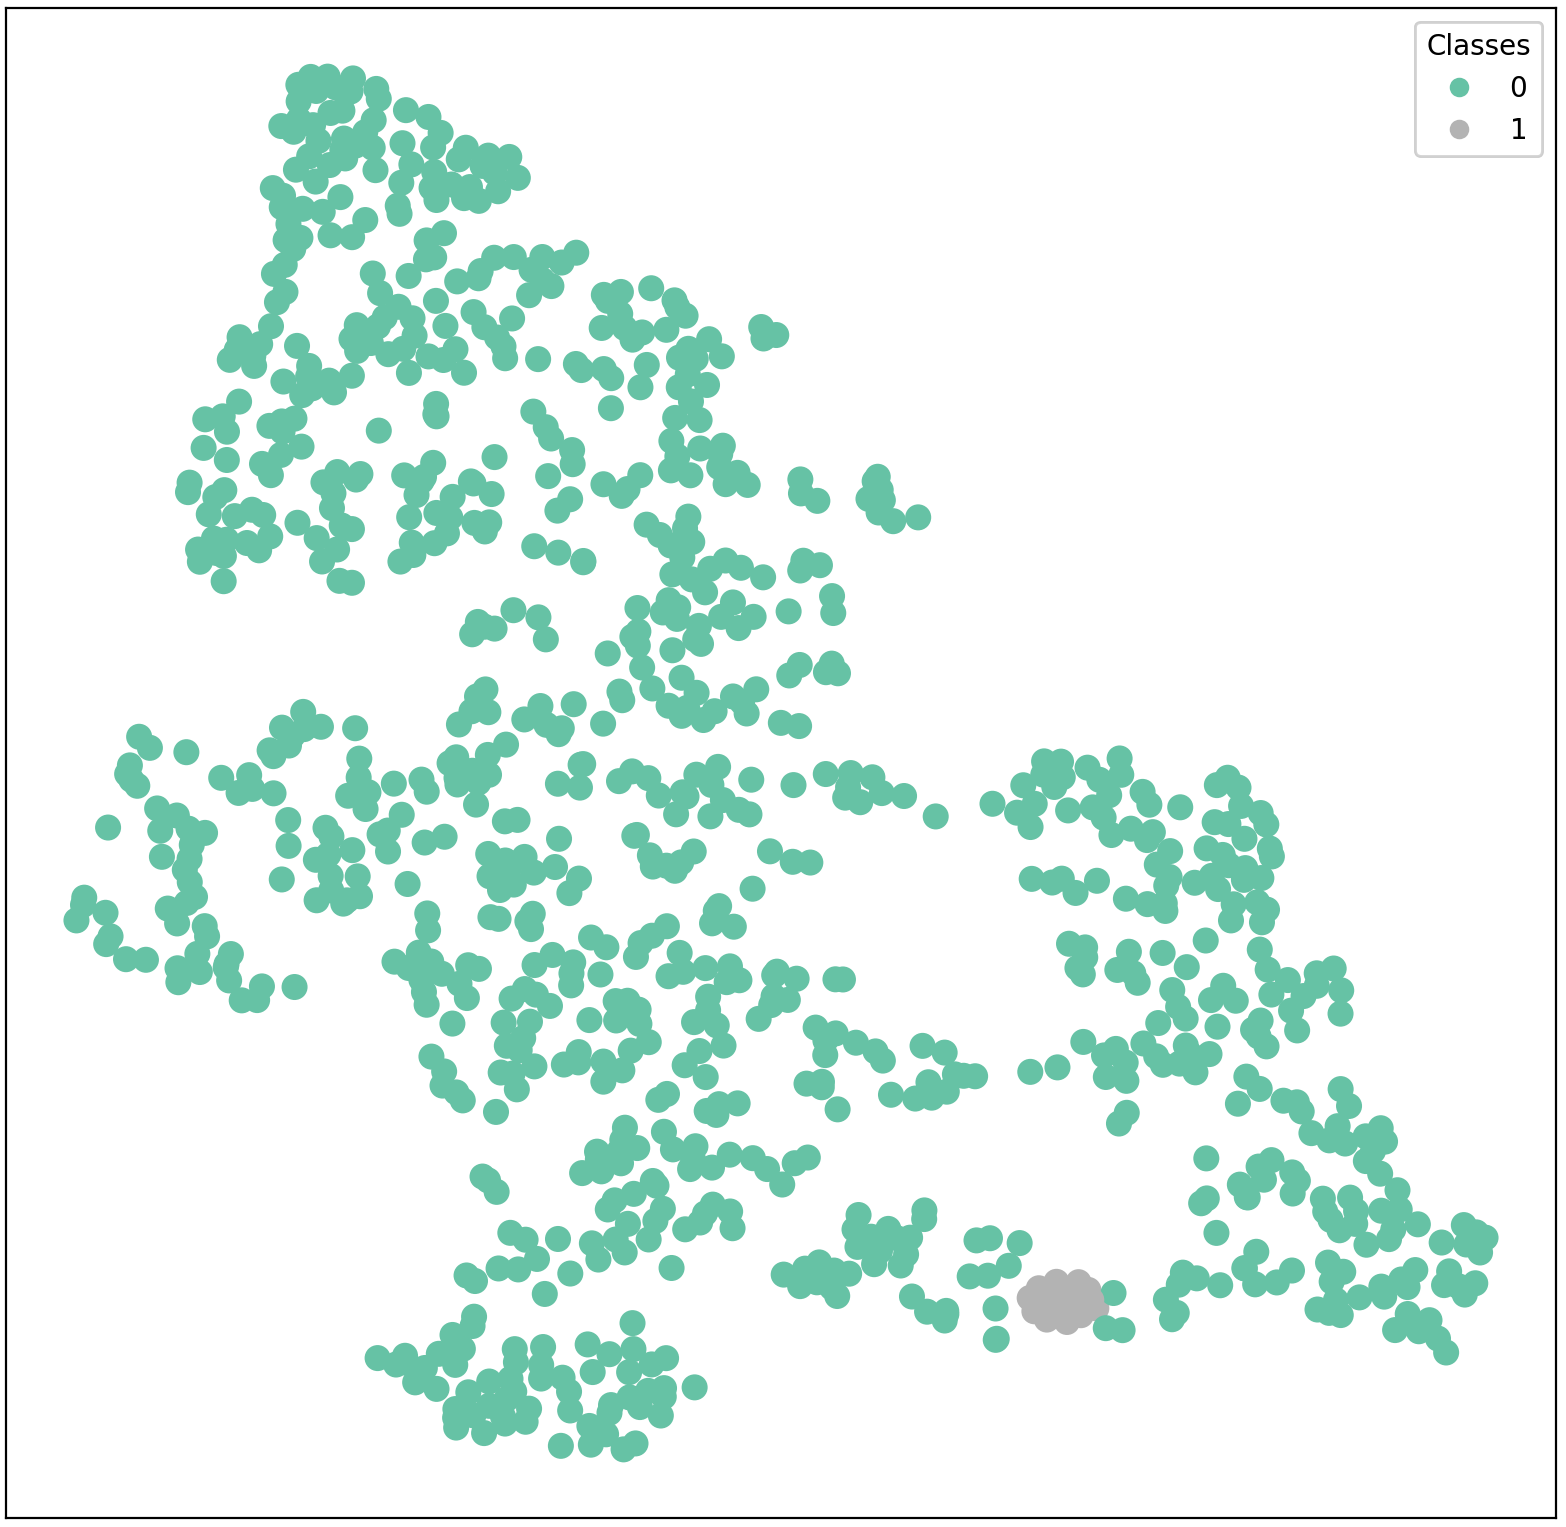
\includegraphics[width=\linewidth]{gcd-test-medium-tsne-after.png}
    \caption{TSNE for TS2 (naive edge weights) after.}
  \end{minipage}
  \begin{minipage}{0.32\textwidth}
    \centering
    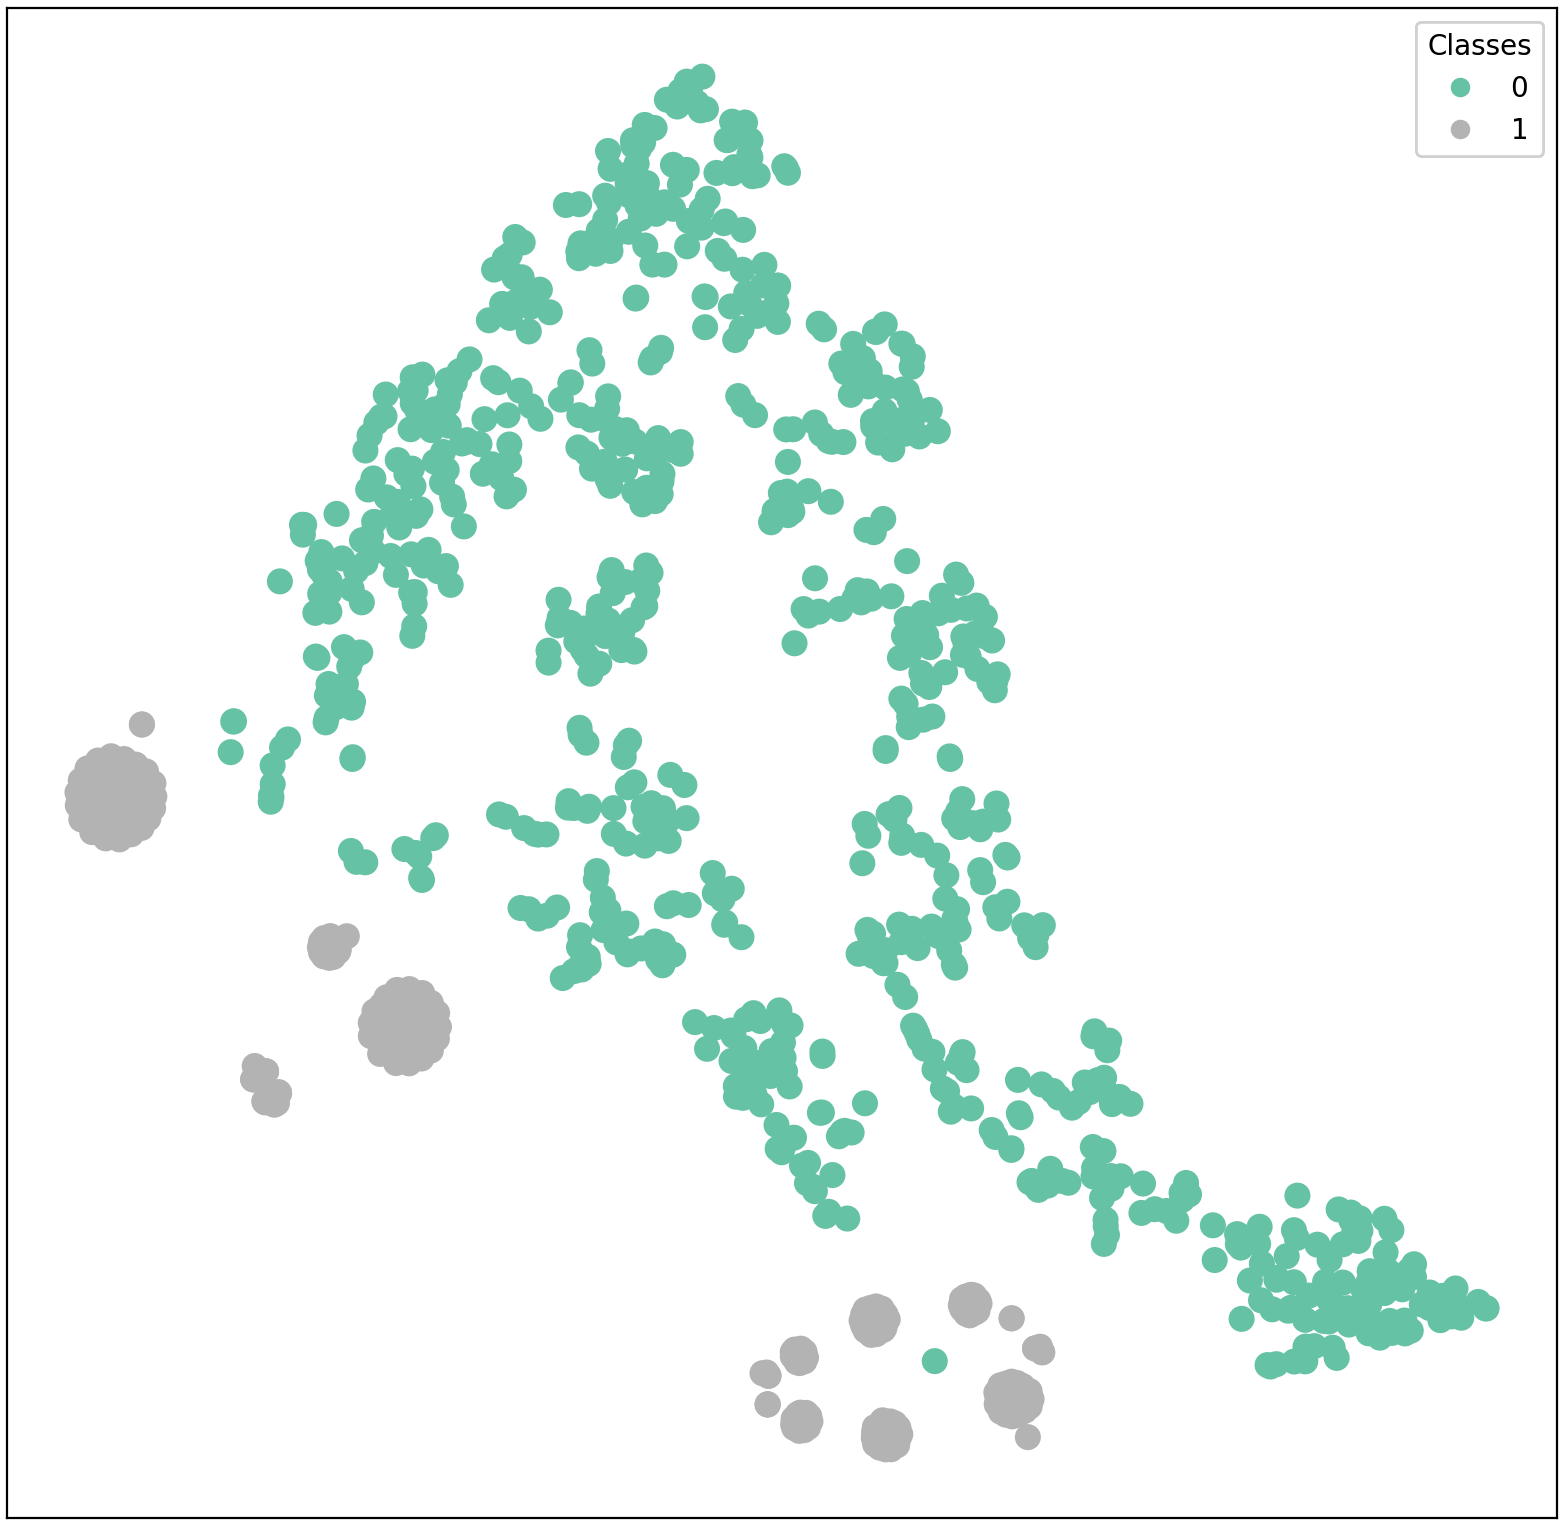
\includegraphics[width=\linewidth]{gcd-test-high-tsne-after.png}
    \caption{TSNE for TS3 (naive edge weights) after.}
  \end{minipage}
  \begin{minipage}{0.32\textwidth}
    \centering
    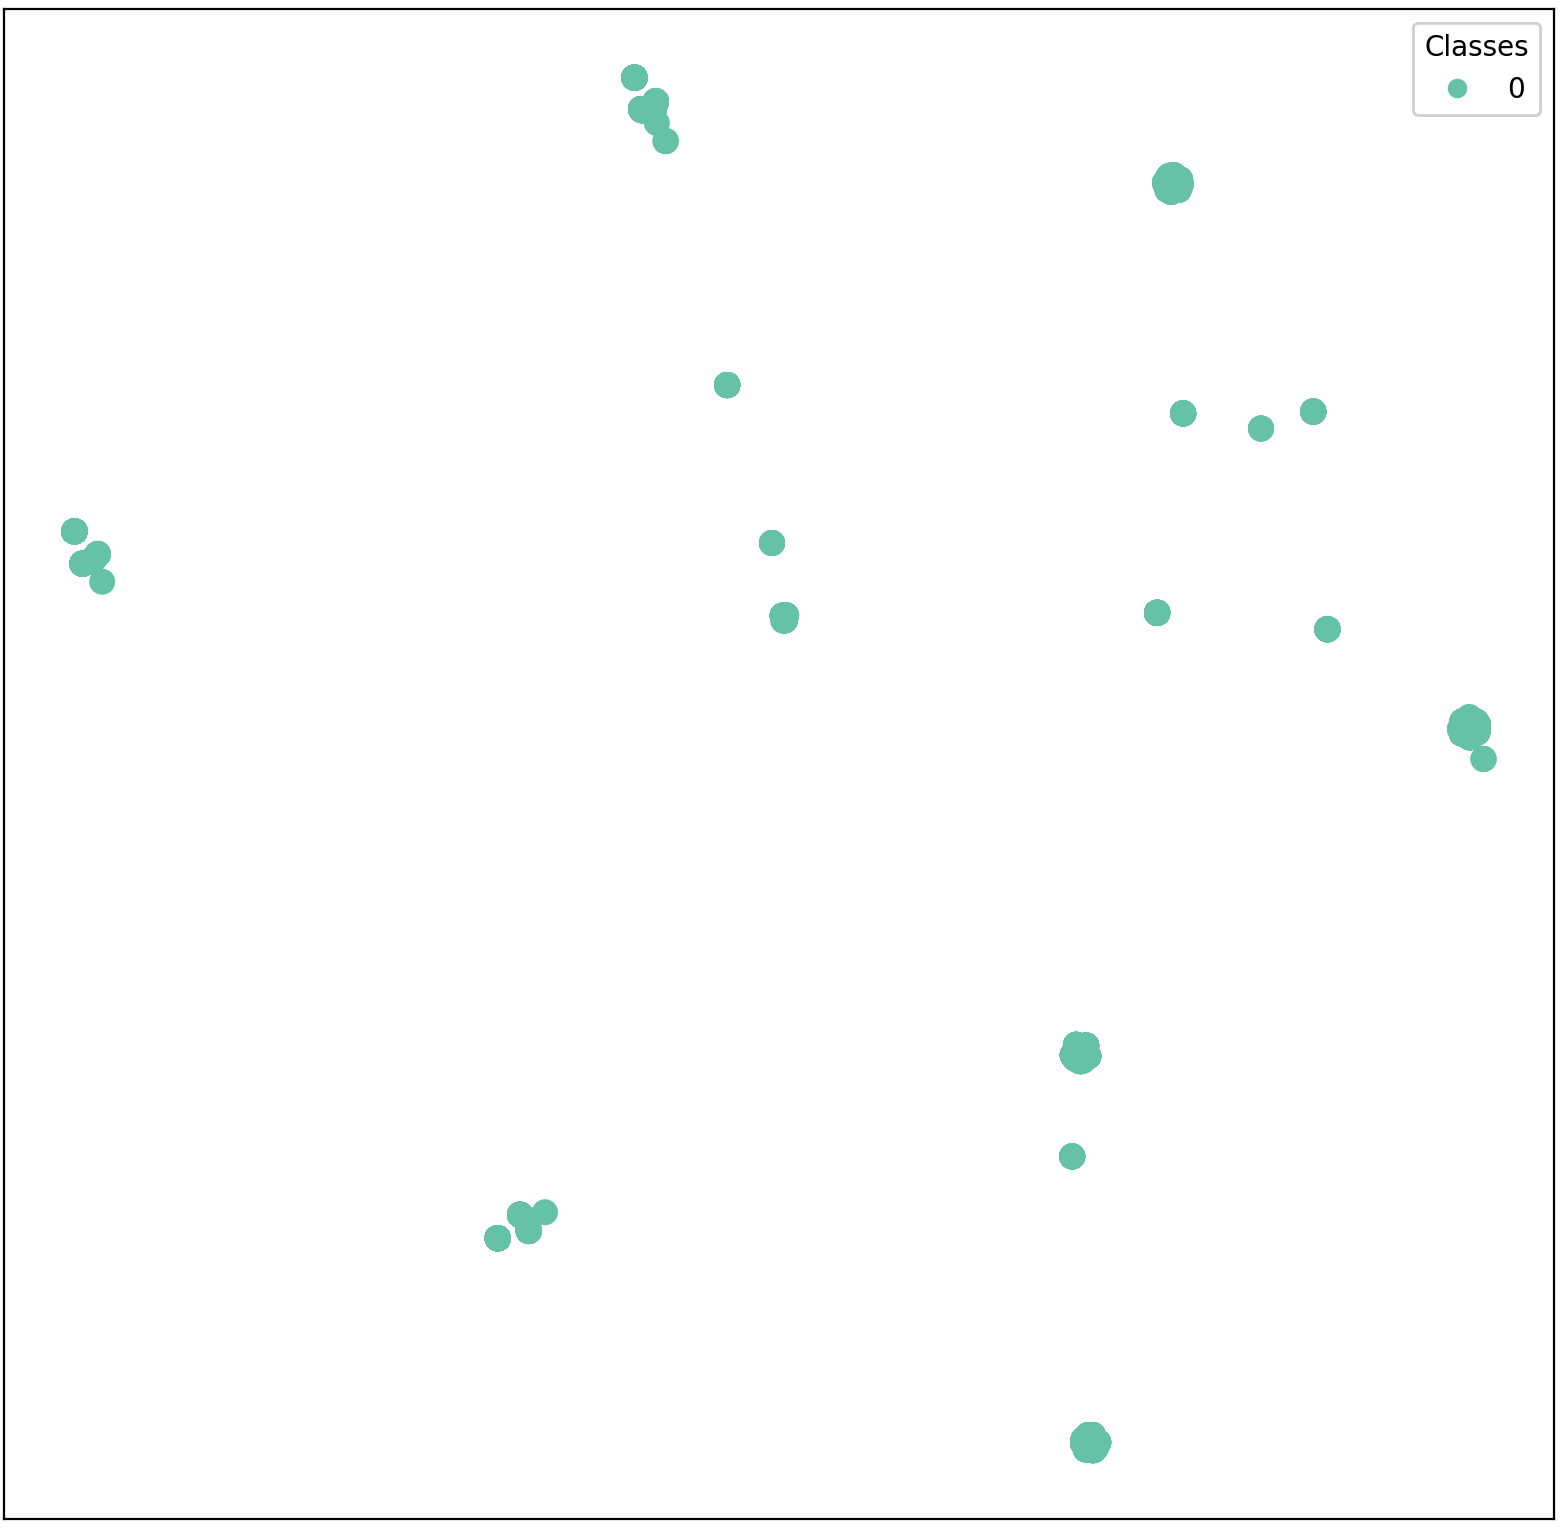
\includegraphics[width=\linewidth]{gcd-adv-test-no-tsne-after.png}
    \caption{TSNE for TS1 (advanced edge weights) after.}
  \end{minipage}
  \begin{minipage}{0.32\textwidth}
    \centering
    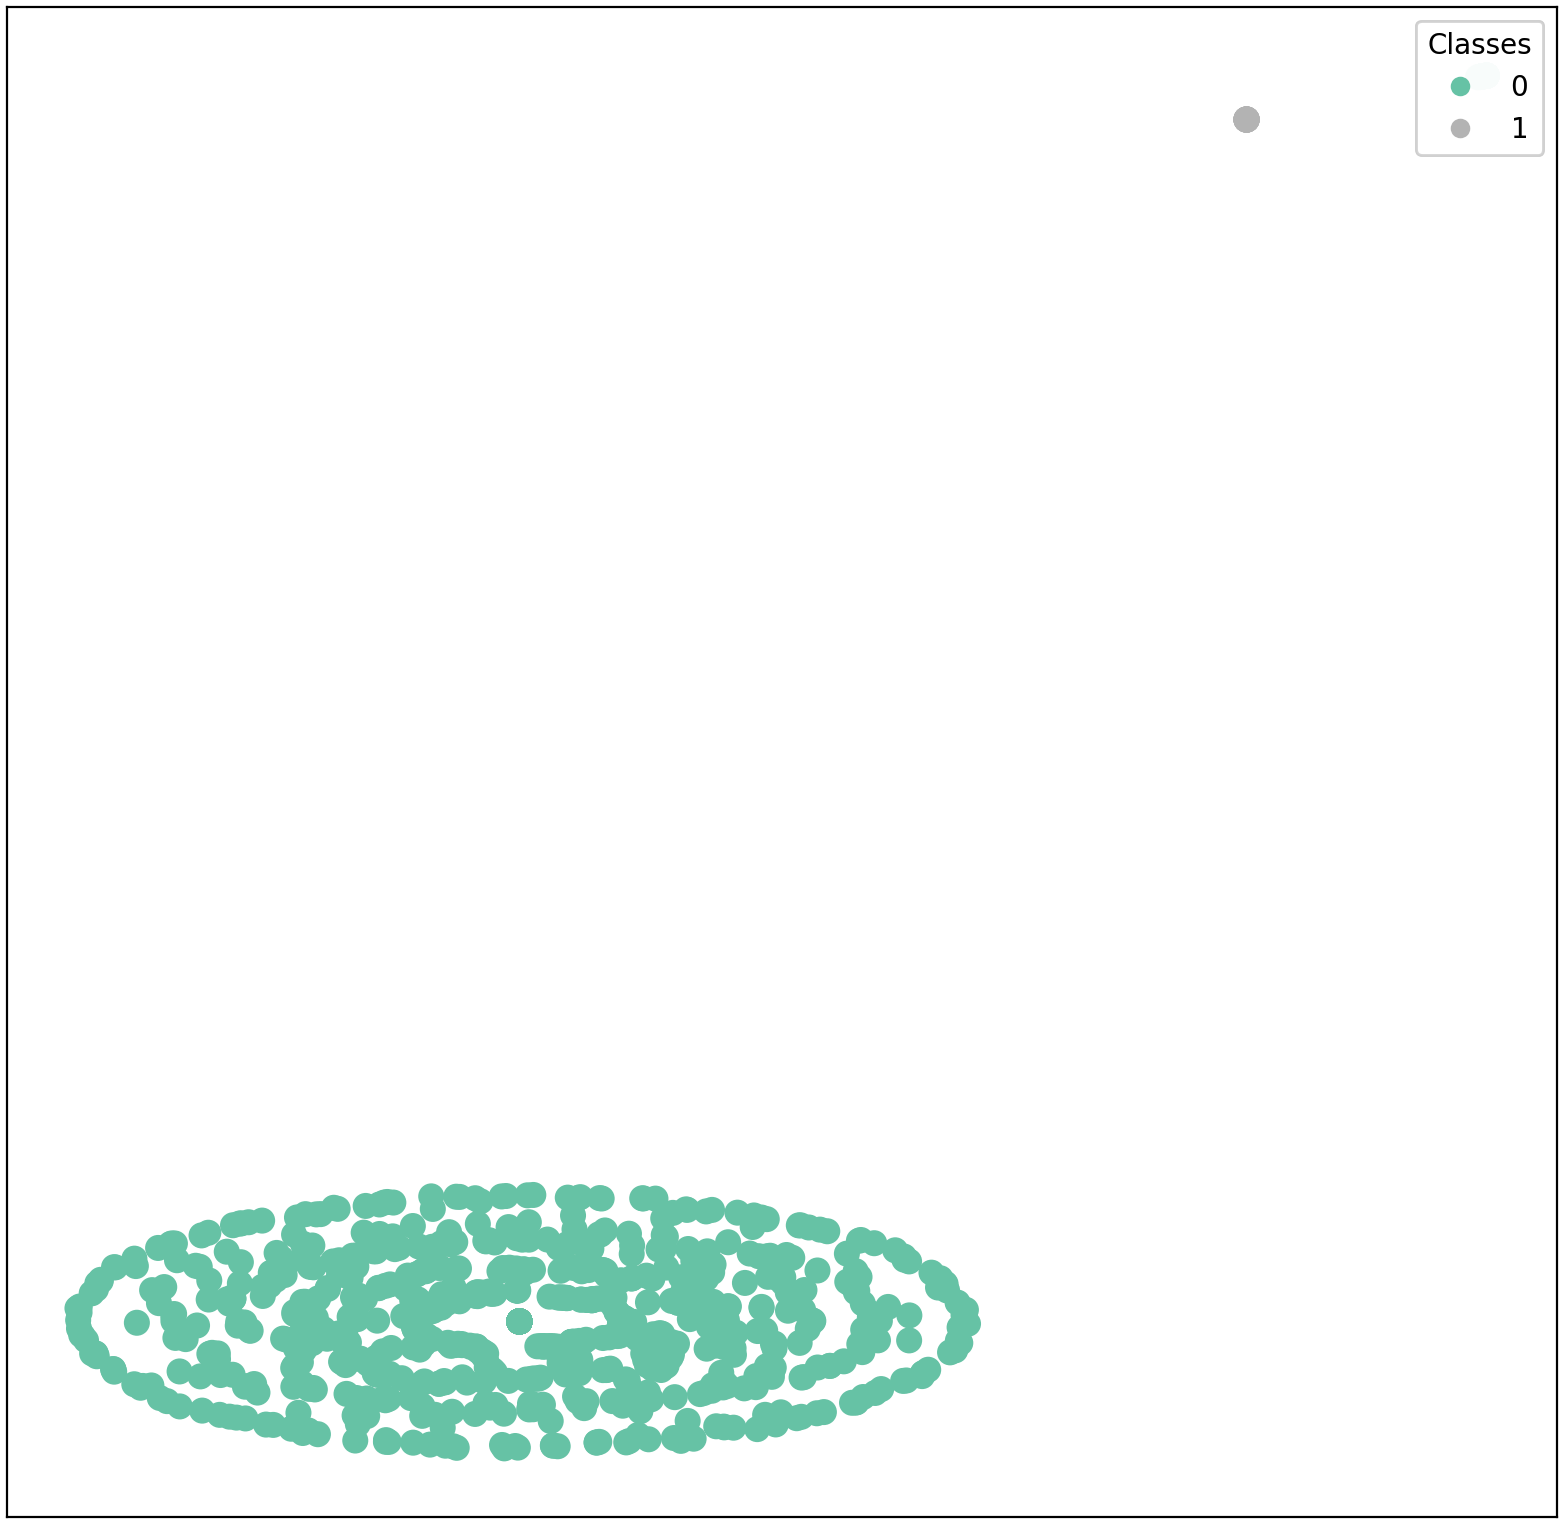
\includegraphics[width=\linewidth]{gcd-adv-test-medium-tsne-after.png}
    \caption{TSNE for TS2 (advanced edge weights) after.}
  \end{minipage}
  \begin{minipage}{0.32\textwidth}
    \centering
    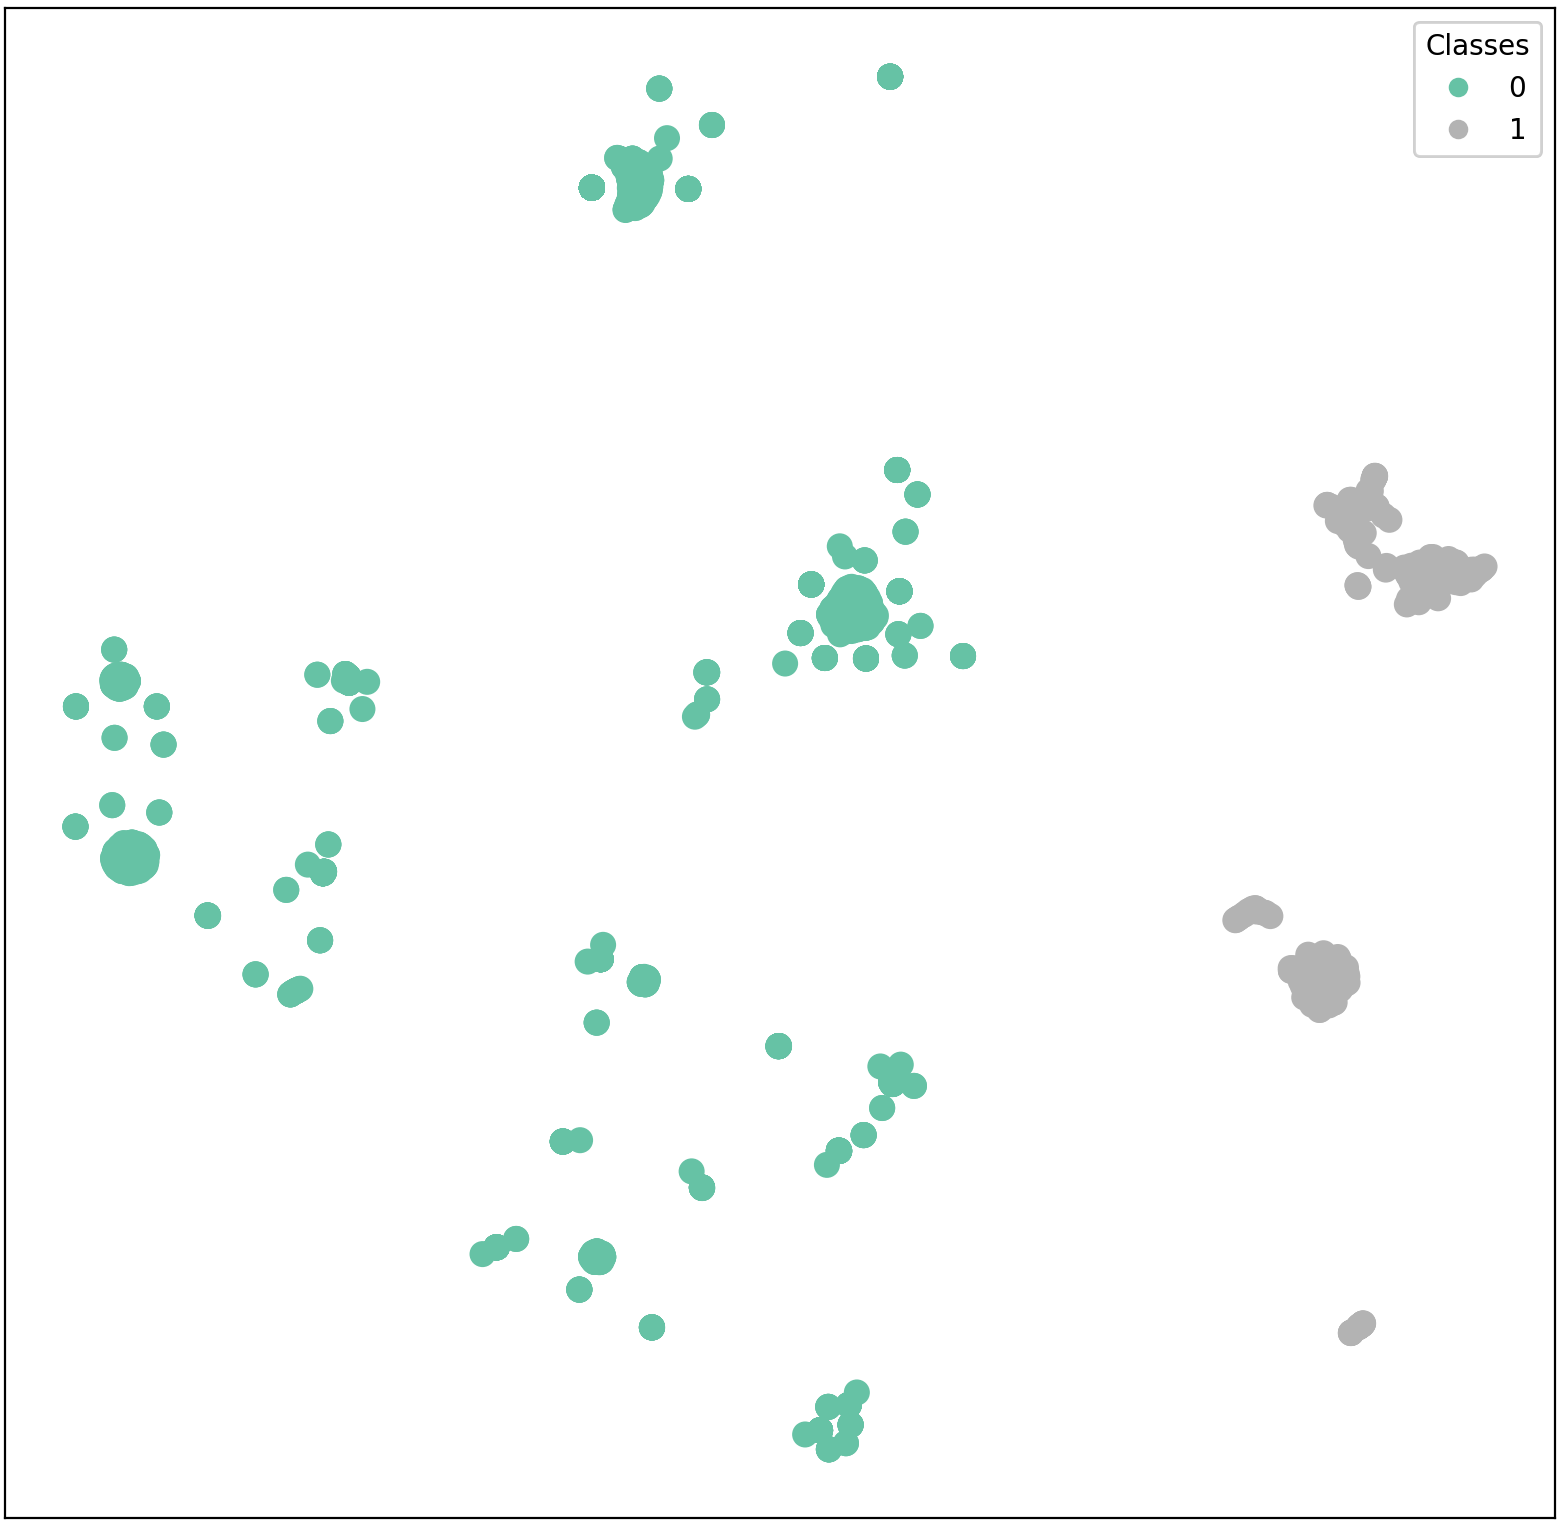
\includegraphics[width=\linewidth]{gcd-adv-test-high-tsne-after.png}
    \caption{TSNE for TS3 (advanced edge weights) after.}
  \end{minipage}
  \caption{TSNE for GCN Test Datasets with naive edge weights.}
  \label{fig:gcn-test-tsne}
\end{figure}

% ---------------------------------------------------------------------------
% ----------------------- end of thesis sub-document ------------------------
% ---------------------------------------------------------------------------
